\section*{Preface}
This chapter is about discovering a material which achieved one of the highest specific capacities for non-aqueous aluminium-ion batteries! Boron nitride was tested as a cathode material and it showed a very high discharge capacity (>250 mAh g$^{-1}$). However, it turned out that boric anhydride (\ce{B2O3}), which was an impurity in hexagonal boron nitride (hBN), was the active material. Pure \ce{B2O3} was tested as a cathode material, the battery produced a similar discharge capacity of >250 mAh g$^{-1}$.   

\begin{figure}[tbh!]
\centering
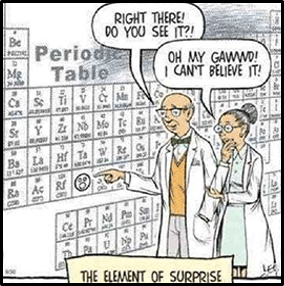
\includegraphics[width=\textwidth]{Figures/BOhBN/ah}
\end{figure}

\newpage
\chapter{Boron nitride/boron oxide as a cathode for rechargeable AIBs} 
\label{BOhBN} 

\section{Theory and background}

\begin{figure}[tbh!]
\centering
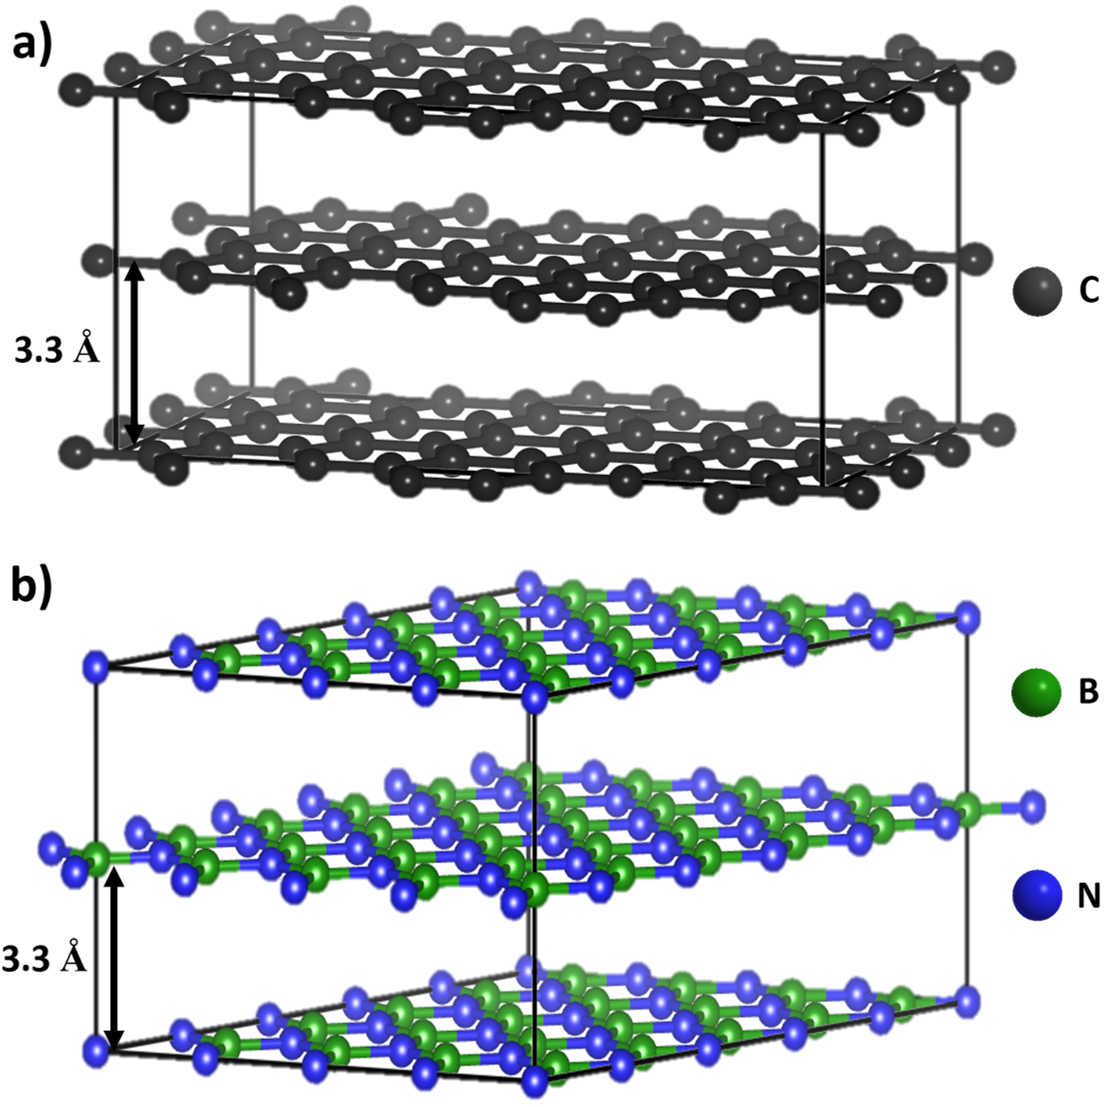
\includegraphics[width=\textwidth]{Figures/BOhBN/grpBNcomp}
\caption{Honeycomb lattice of a) natural graphite and b) hexagonal boron nitride. Both structures display an interlayer distance of 3.3\AA.}
\label{Figures/BOhBN:grpBNcomp}
\end{figure}

Graphite has been extensively used as a cathode in AIBs due to its high conductivity and its layered structure. Graphite and hexagonal boron nitride (hBN) are materials that possess a hexagonal lattice structure \cite{hod_graphite_2012}. hBN is also known as inorganic graphite. Where graphite has non-polar homonuclear C-C intralayer bonds, hBN on the other hand displays highly polar B-N bonds. In the bulk form, the two materials have different stacking modes. Furthermore, the static polarizabilities of the constituent atoms are significantly different, suggesting large differences in the dispersive component of the interlayer bonding\cite{song_large_2010, zeng_white_2010}. Despite these major differences, both materials present practically identical interlayer distances as shown in  Figure \ref{Figures/BOhBN:grpBNcomp}. Structurally, a single layer of hBN is very similar to a graphene sheet and has a hexagonal backbone where each couple of bonded carbon atoms is replaced by a boron nitride pair, making the two materials isoelectronic. Nevertheless, due to the electronegativity differences between the boron and the nitrogen atoms, the $\pi$ electrons tend to localize around the nitrogen atomic centers, thus making it an insulating material. The nature of bonding between nitrogen and boron differs from the carbon-carbon bonds found in graphite. hBN possesses coordinate bonds resulting from donation of \ce{e-} pair from nitrogen into empty p-orbital of a neighbouring B atom. Each N atom develops a partial positive charge and each B develops a partial negative charge. The partial ionic character of BN bonding makes it a semi-conductor as opposed to a conductor like graphite. hBN has been used in solid-state LIBs in various forms. When it is mixed with the electrolyte, it imparts exceptional thermal stability that allows high-rate operation of solid-state rechargeable LIBs at temperatures up to 175 $^{\circ}$C\cite{hyun_high}. When coated onto the surface of a poly(ethylene oxide) (PEO)-based electrolyte, hBN formed a robust interfacial layer to improve the chemical and mechanical stability of the PEO-based electrolyte, leading to the enhanced performance of solid-state Li metal batteries\cite{shen_chem}. Boron nitride nanotubes (BNNTs) were synthesized by Rahman \textit{et al.} and used for the modification of a polyolefin separator without blocking the porous channels of the conventional separator for \ce{Li+} ion diffusion. This improved the thermal stability up to 150 $^{\circ}$C \cite{rahamn_}.\\*
For the above mentioned advantages, hBN was considered as a cathode for AIBs. Despite the fact that hBN is an insulator, it was assumed that additives like conductive carbon (Super-P) would compensate for the loss of conductivity. In addition, hBN was a new material in the field of AIBs.\\* 

\section{Results and discussion}

\begin{figure}[tbh!]
\centering
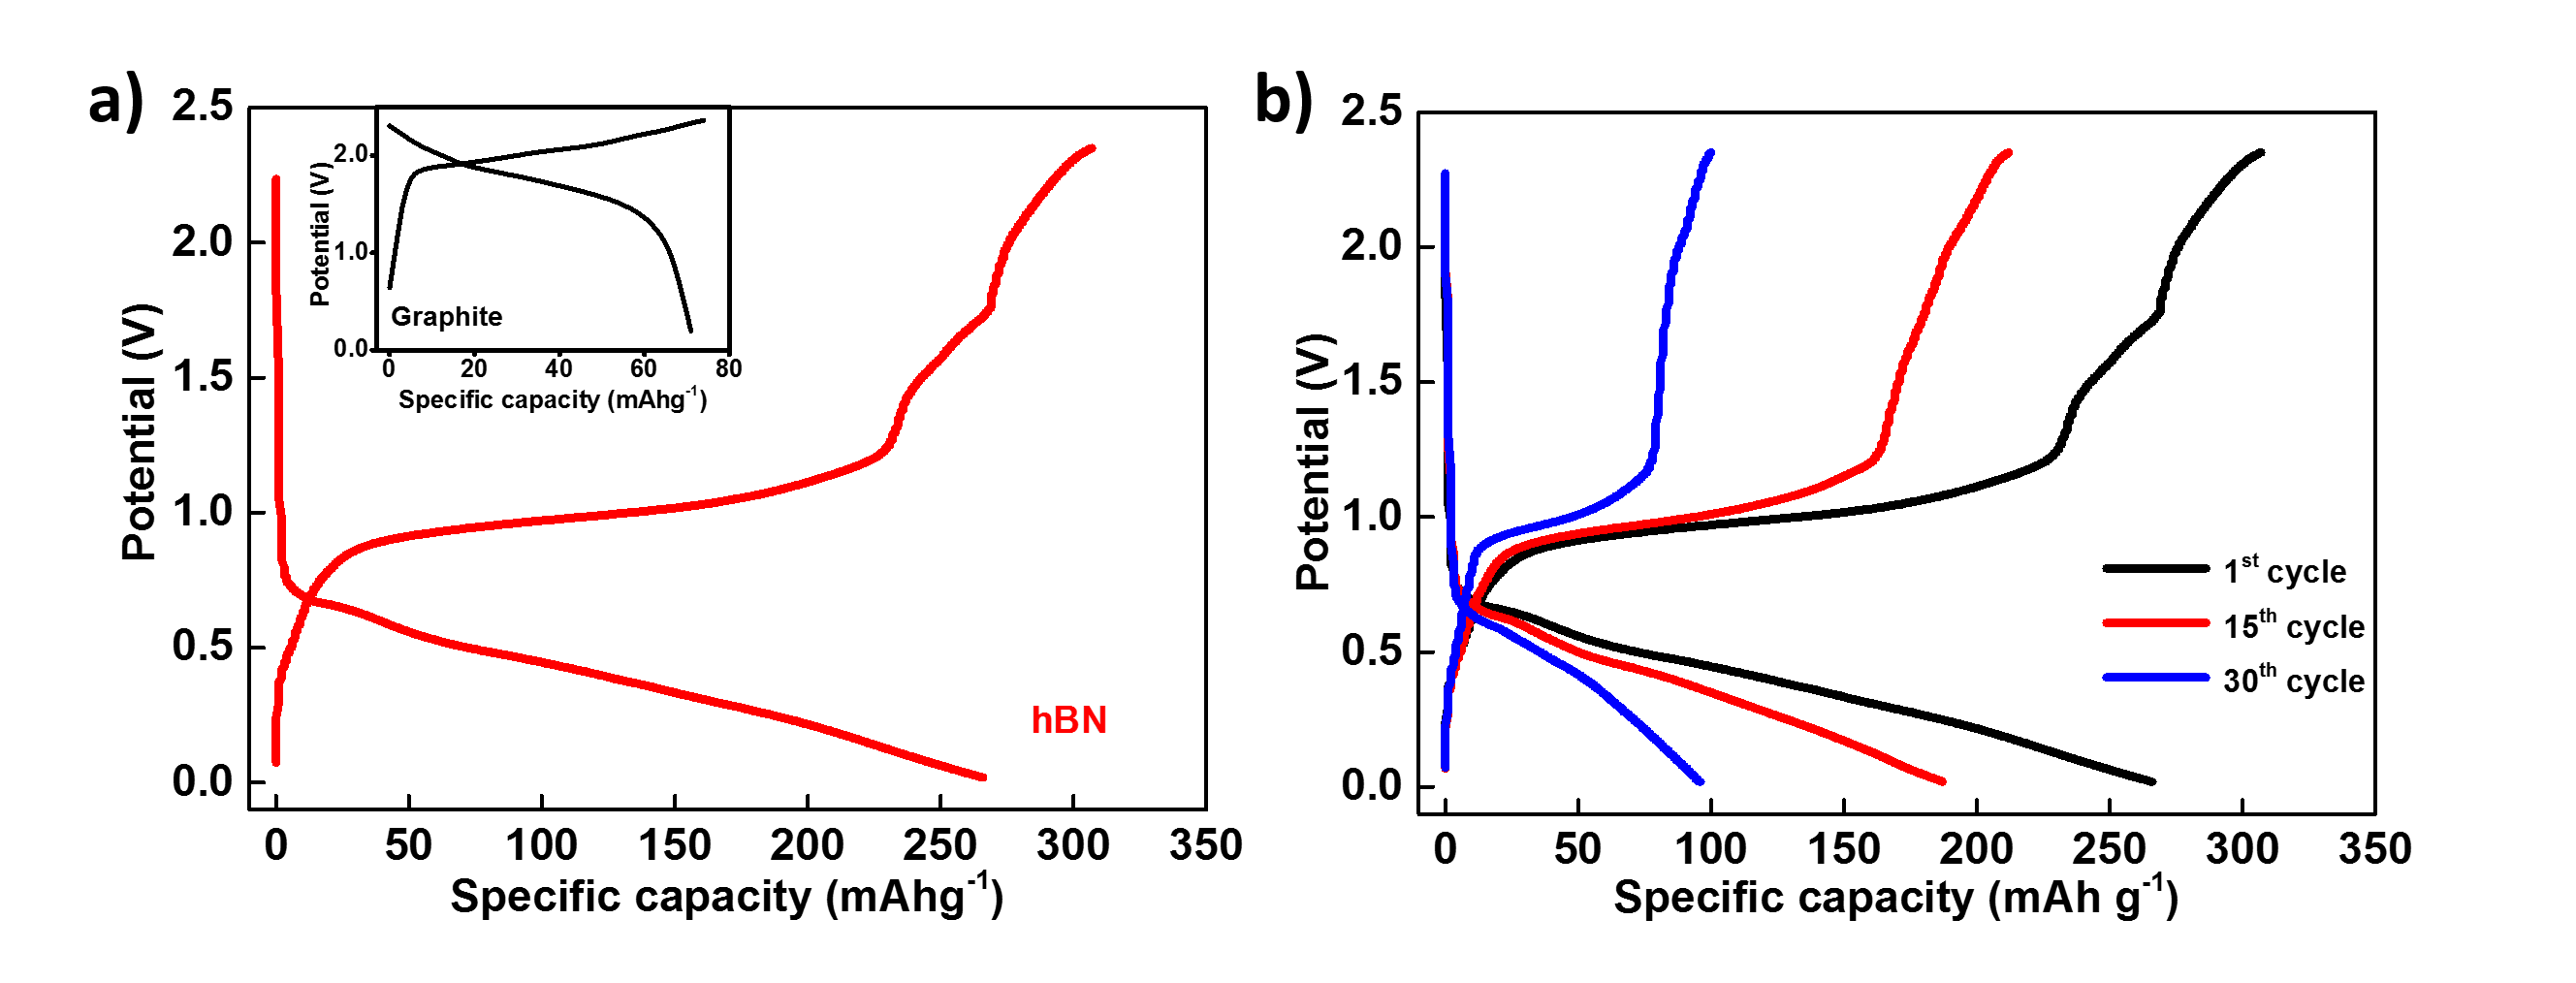
\includegraphics[width=\textwidth]{Figures/BOhBN/hBNiniCDC}
\caption{a) Galvanostatic cycles of an Al/hBN, using hBN from the stores (with \ce{B2O3} as an impurity), at a current density of 50 mA g$^{-1}$ compared with natural graphite (inset). b) Capacity fading of Al/hBN cell recorded for 30 cycles at a current rate of 50 mA g$^{-1}$.}
\label{Figures/BOhBN:hBNiniCDC}
\end{figure}

\begin{figure}[tbh!]
\centering
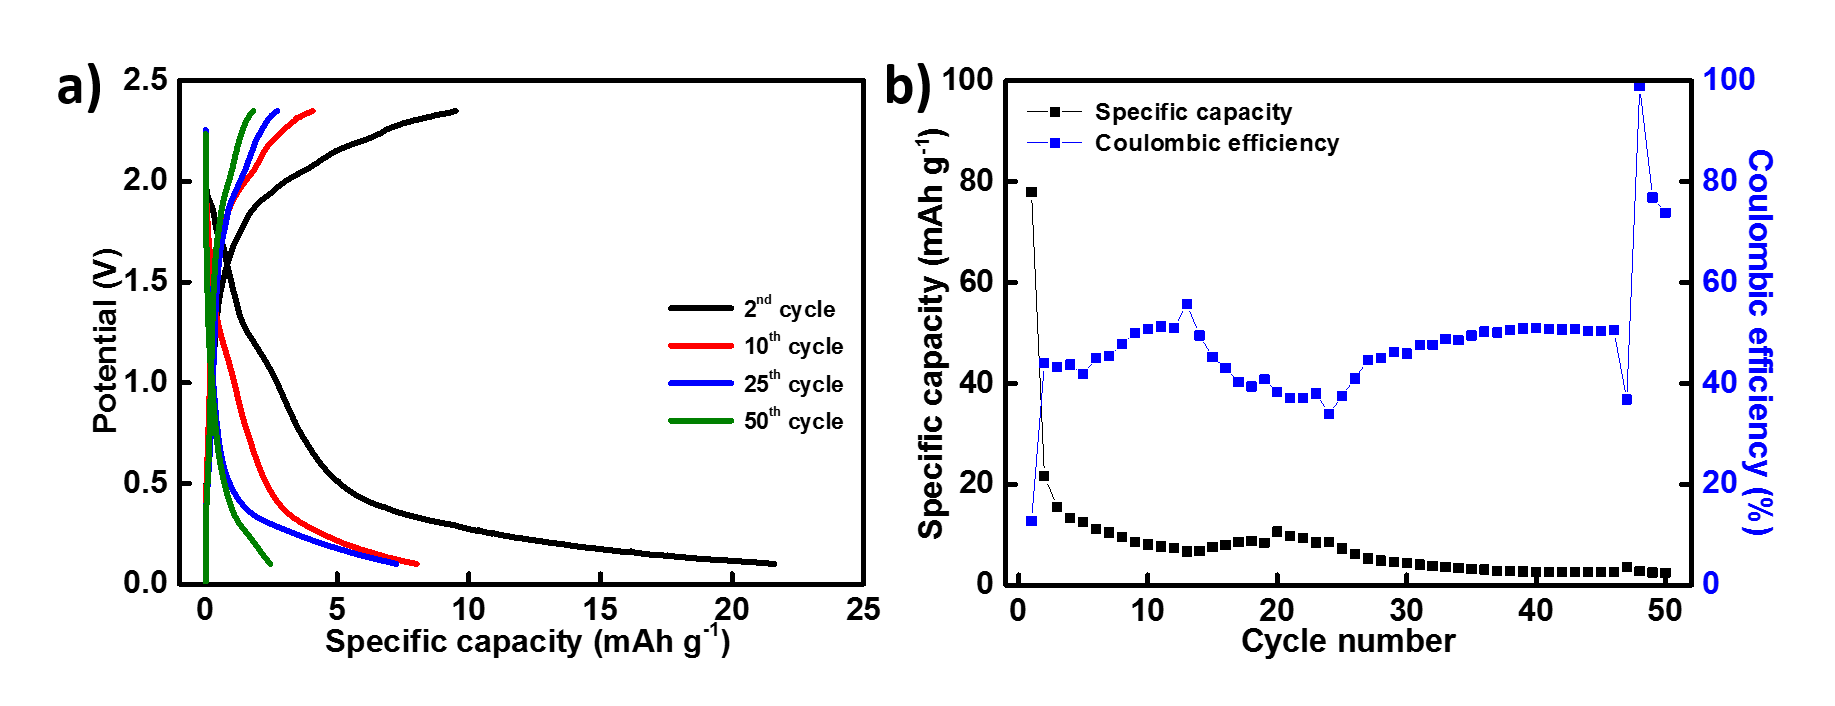
\includegraphics[width=\textwidth]{Figures/BOhBN/BNNSCDCCE}
\caption{a) Performance of an aluminium-ion battery using pure hBN as cathode at a current rate of 50 mA g$^{-1}$. b) Discharge capacity drops down to 5 mAh g$^{-1}$ after 50 cycles. hBN displays a very low coulombic efficiency $\approx$ 55\%.}
\label{Figures/BOhBN:hBNCDCCE}
\end{figure}

For all the above mentioned reasons, we tested hBN as a cathode for AIBs. To save cost, an old bottle of hBN was retrieved from VUW's chemical stores. A cell was assembled and preliminary electrochemical tests were performed. Figure \ref{Figures/BOhBN:hBNiniCDC} displays the galvanostatic charge/discharge profile of an Al/hBN cell at a current density of 50 mA g$^{-1}$. hBN exhibited very high specific capacities reaching values as high as 270 mAh g$^{-1}$. The cell displayed a discharge potential of 0.6 V. Despite being not as conductive as graphite, the discharge capacity value was more than three times the capacity of graphite (inset, Figure \ref{Figures/BOhBN:hBNiniCDC}a). Repeated measurements of Al/hBN cells using hBN from the same old bottle of hBN gave similar results, Figure \ref{Figures/appendix:hBNrepeat}. However, it was noted that the specific capacity dropped after a few cycles. In Figure \ref{Figures/BOhBN:hBNiniCDC}b, it was observed that the capacity retention of hBN was very poor (decreased by 60\%) after 30 cycles. In expectation of better results, a new bottle of hBN from Sigma Aldrich (98\%, $\sim$1 $\mu$m in size) was purchased. New batch of cathodes were made and tested. Surprisingly, the discharge capacity obtained from the new cells was nowhere near the values achieved by the older hBN as displayed in Figure \ref{Figures/BOhBN:hBNCDCCE}. A number of batches were made from the new bottle, but none of them achieved capacities higher than 50 mAh g$^{-1}$ (Figure \ref{Figures/appendix:hBNmultiattempts}). It seemed that two completely different materials were being tested! Given the old nature of the hBN sample, it was important to investigate whether the material was actually hBN or had it changed to some other compound over time.\\*
Figure \ref{Figures/BOhBN:oldxps} displays the binding energy of 1s orbital of boron. Th experimental peak was split into two peaks after curve fitting. In addition, with the B-N bond, a new B-O bond with a binding energy at 193.5 eV was observed. This suggested a strong presence of a \ce{B2O3} in the old hBN sample.
\begin{figure}[tbh!]
\centering
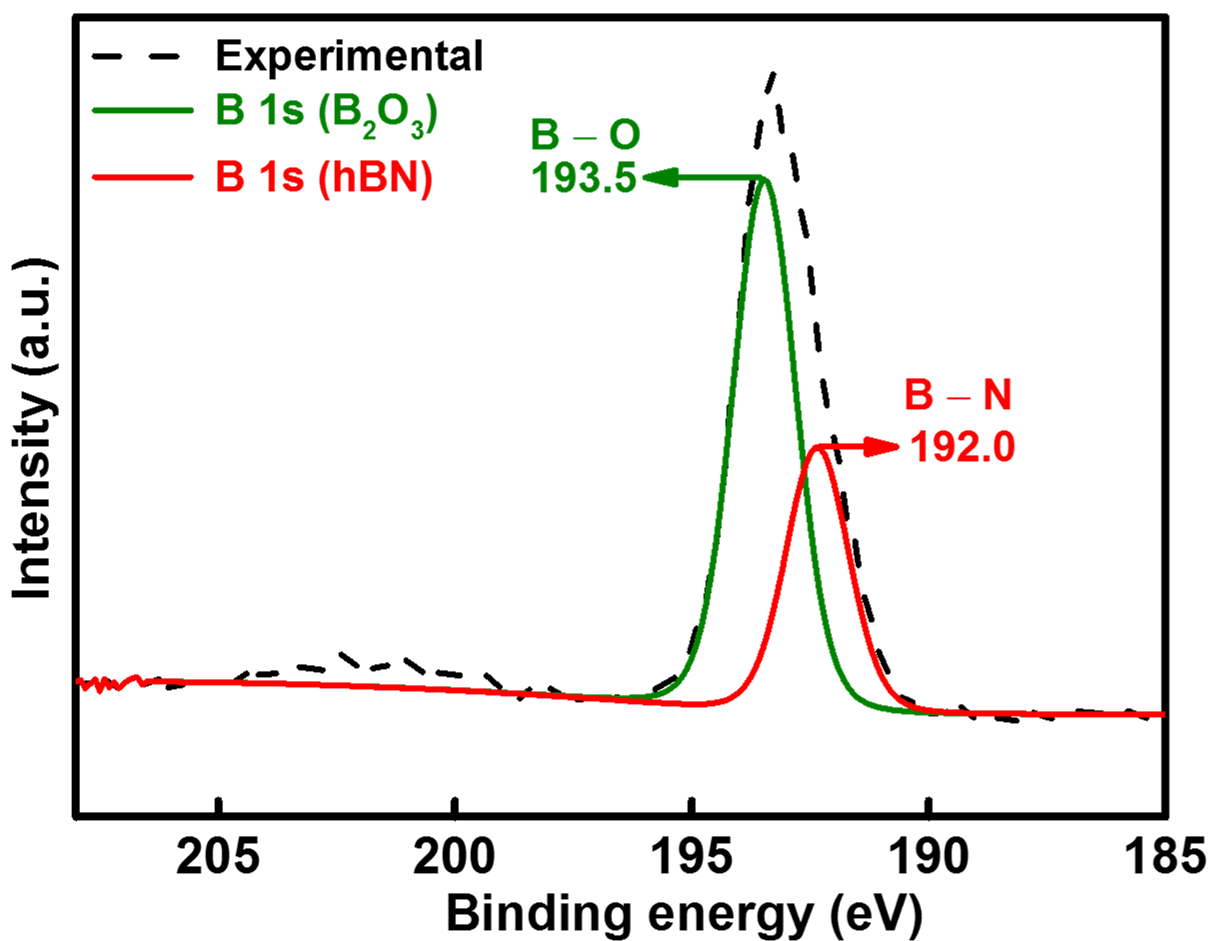
\includegraphics[width=\textwidth]{Figures/BOhBN/oldxps}
\caption{X-ray photoelectron spectra an old hBN cathode.}
\label{Figures/BOhBN:oldxps}
\end{figure}

To conclude that hBN did not play any active role in the old sample cell, boron nitride nano sheets (BNNS) were synthesised and tested as cathodes for AIBs. 
\large{Boron nitride nano sheets (BNNS)}
As mentioned in previous chapters, nano-sized materials increase the contact area between an electrode and electrolyte. They provide short path lengths for both ion diffusion and electron transport, which improves the charge/ discharge rate. The high surface area of the material allows large volume expansion/ contraction associated with ion transport and prevents cathode pulverisation leading to longer cycle-life \cite{zhang_ultrathin_2015,cong_intrinsic_2015}. \\*
\Large{Synthesis of BNNS} \\*
Nano sheets of hexagonal boron nitride were synthesised via mechanical exfoliation. 250 mg of hBN was dispersed in 75 ml isopropanol (IPA) in a 100 ml round bottom flask (RBF). The mixture was heated at 500$^{\circ}$C for 24 hours and was magnetically stirred. To accelerate the dissolution of hBN into IPA, the RBF was then put in an ultrasonic bath for 20 hours. The solution was then left to stand for 2 days and the supernatant was removed in a centrifuge tube. It was centrifuged at a speed of 14000 rpm. The obtained precipitate was washed with acetone to remove residual IPA. The product was dried overnight at 60$^{\circ}$C. 

\begin{figure}[tbh!]
\centering
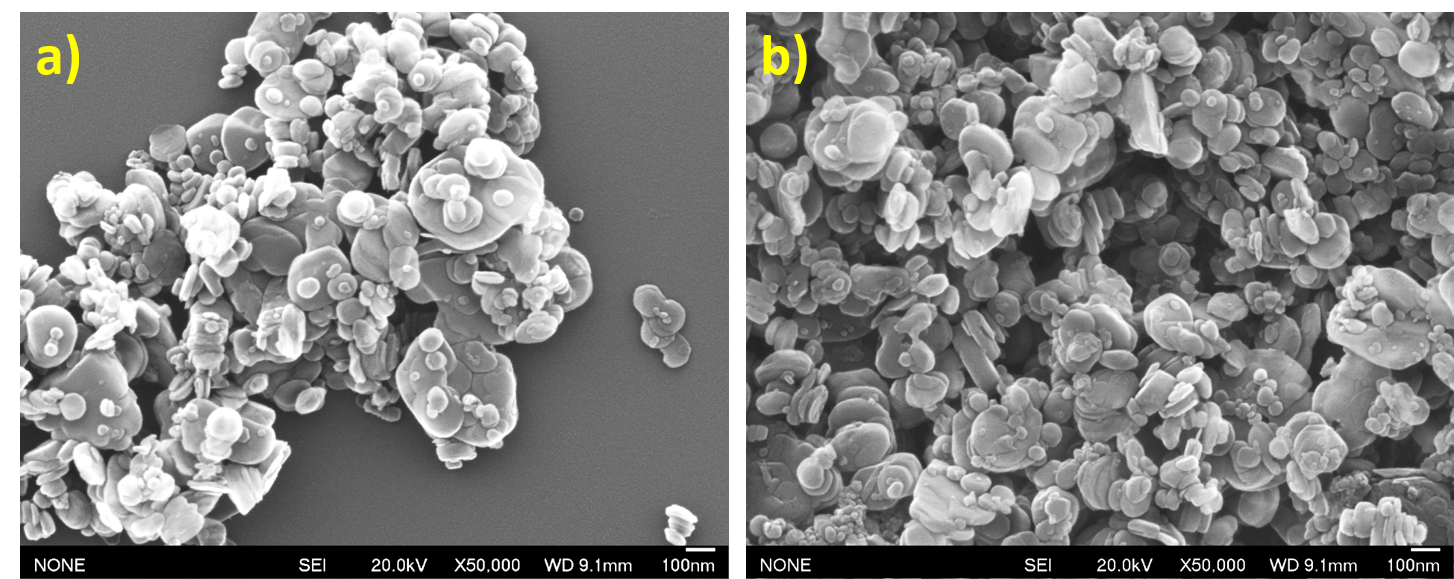
\includegraphics[width=\textwidth]{Figures/BOhBN/BNNSSEM}
\caption{SEM images of hexagonal boron nitride nano sheets.}
\label{Figures/BOhBN:BNNSSEM}
\end{figure}

\begin{figure}[tbh!]
\centering
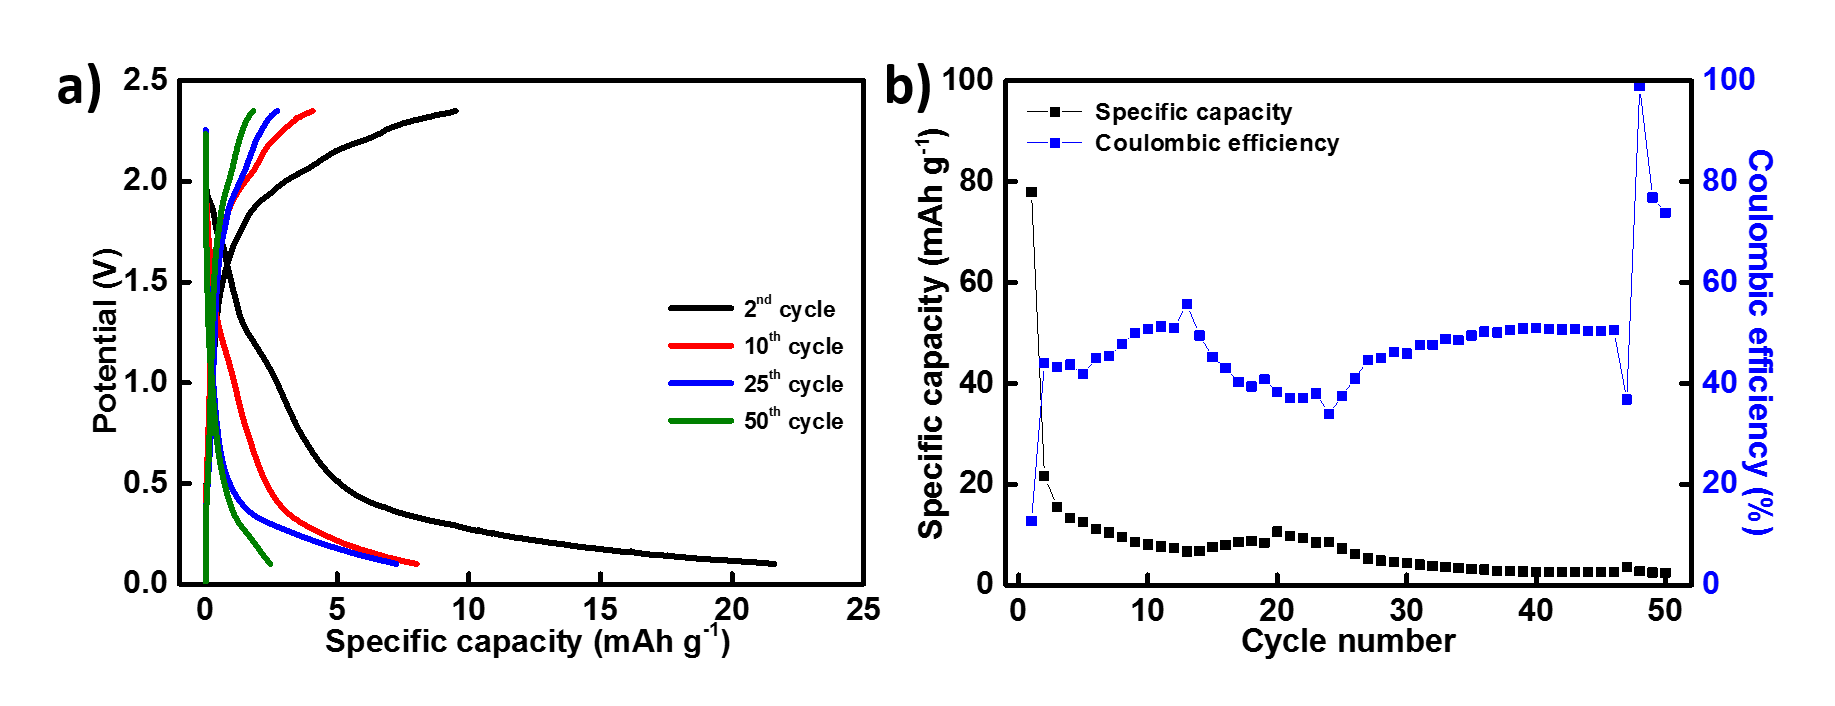
\includegraphics[width=\textwidth]{Figures/BOhBN/BNNSCDCCE}
\caption{Galvanostatic charge/discharge profile of Al/BNNS cell at a current rate of 50 mA g$^{-1}$. The cell achieved 22 mA h g$^{-1}$ in its first cycle, which dropped down to 2 mAh g$^{-1}$ after 50 cycles. Coulombic efficiency was also very low $\sim$50\%. }
\label{Figures/BOhBN:BNNSCDCCE}
\end{figure}

The galvanostatic charge/discharge profile of Al/BNNS is displayed in Figure \ref{Figures/BOhBN:BNNSCDCCE}a and b. Capacity fade and low coulombic efficiencies similar to pure hBN was observed in BNNS as well. This experiment proved that hBN present in the old hBN/\ce{B2O3} mixture, did not have high enough capacity and \ce{B2O3} played a significant role in achieving capacity as high as 270 mAh g$^{-1}$. \\*

\begin{figure}[tbh!]
\centering
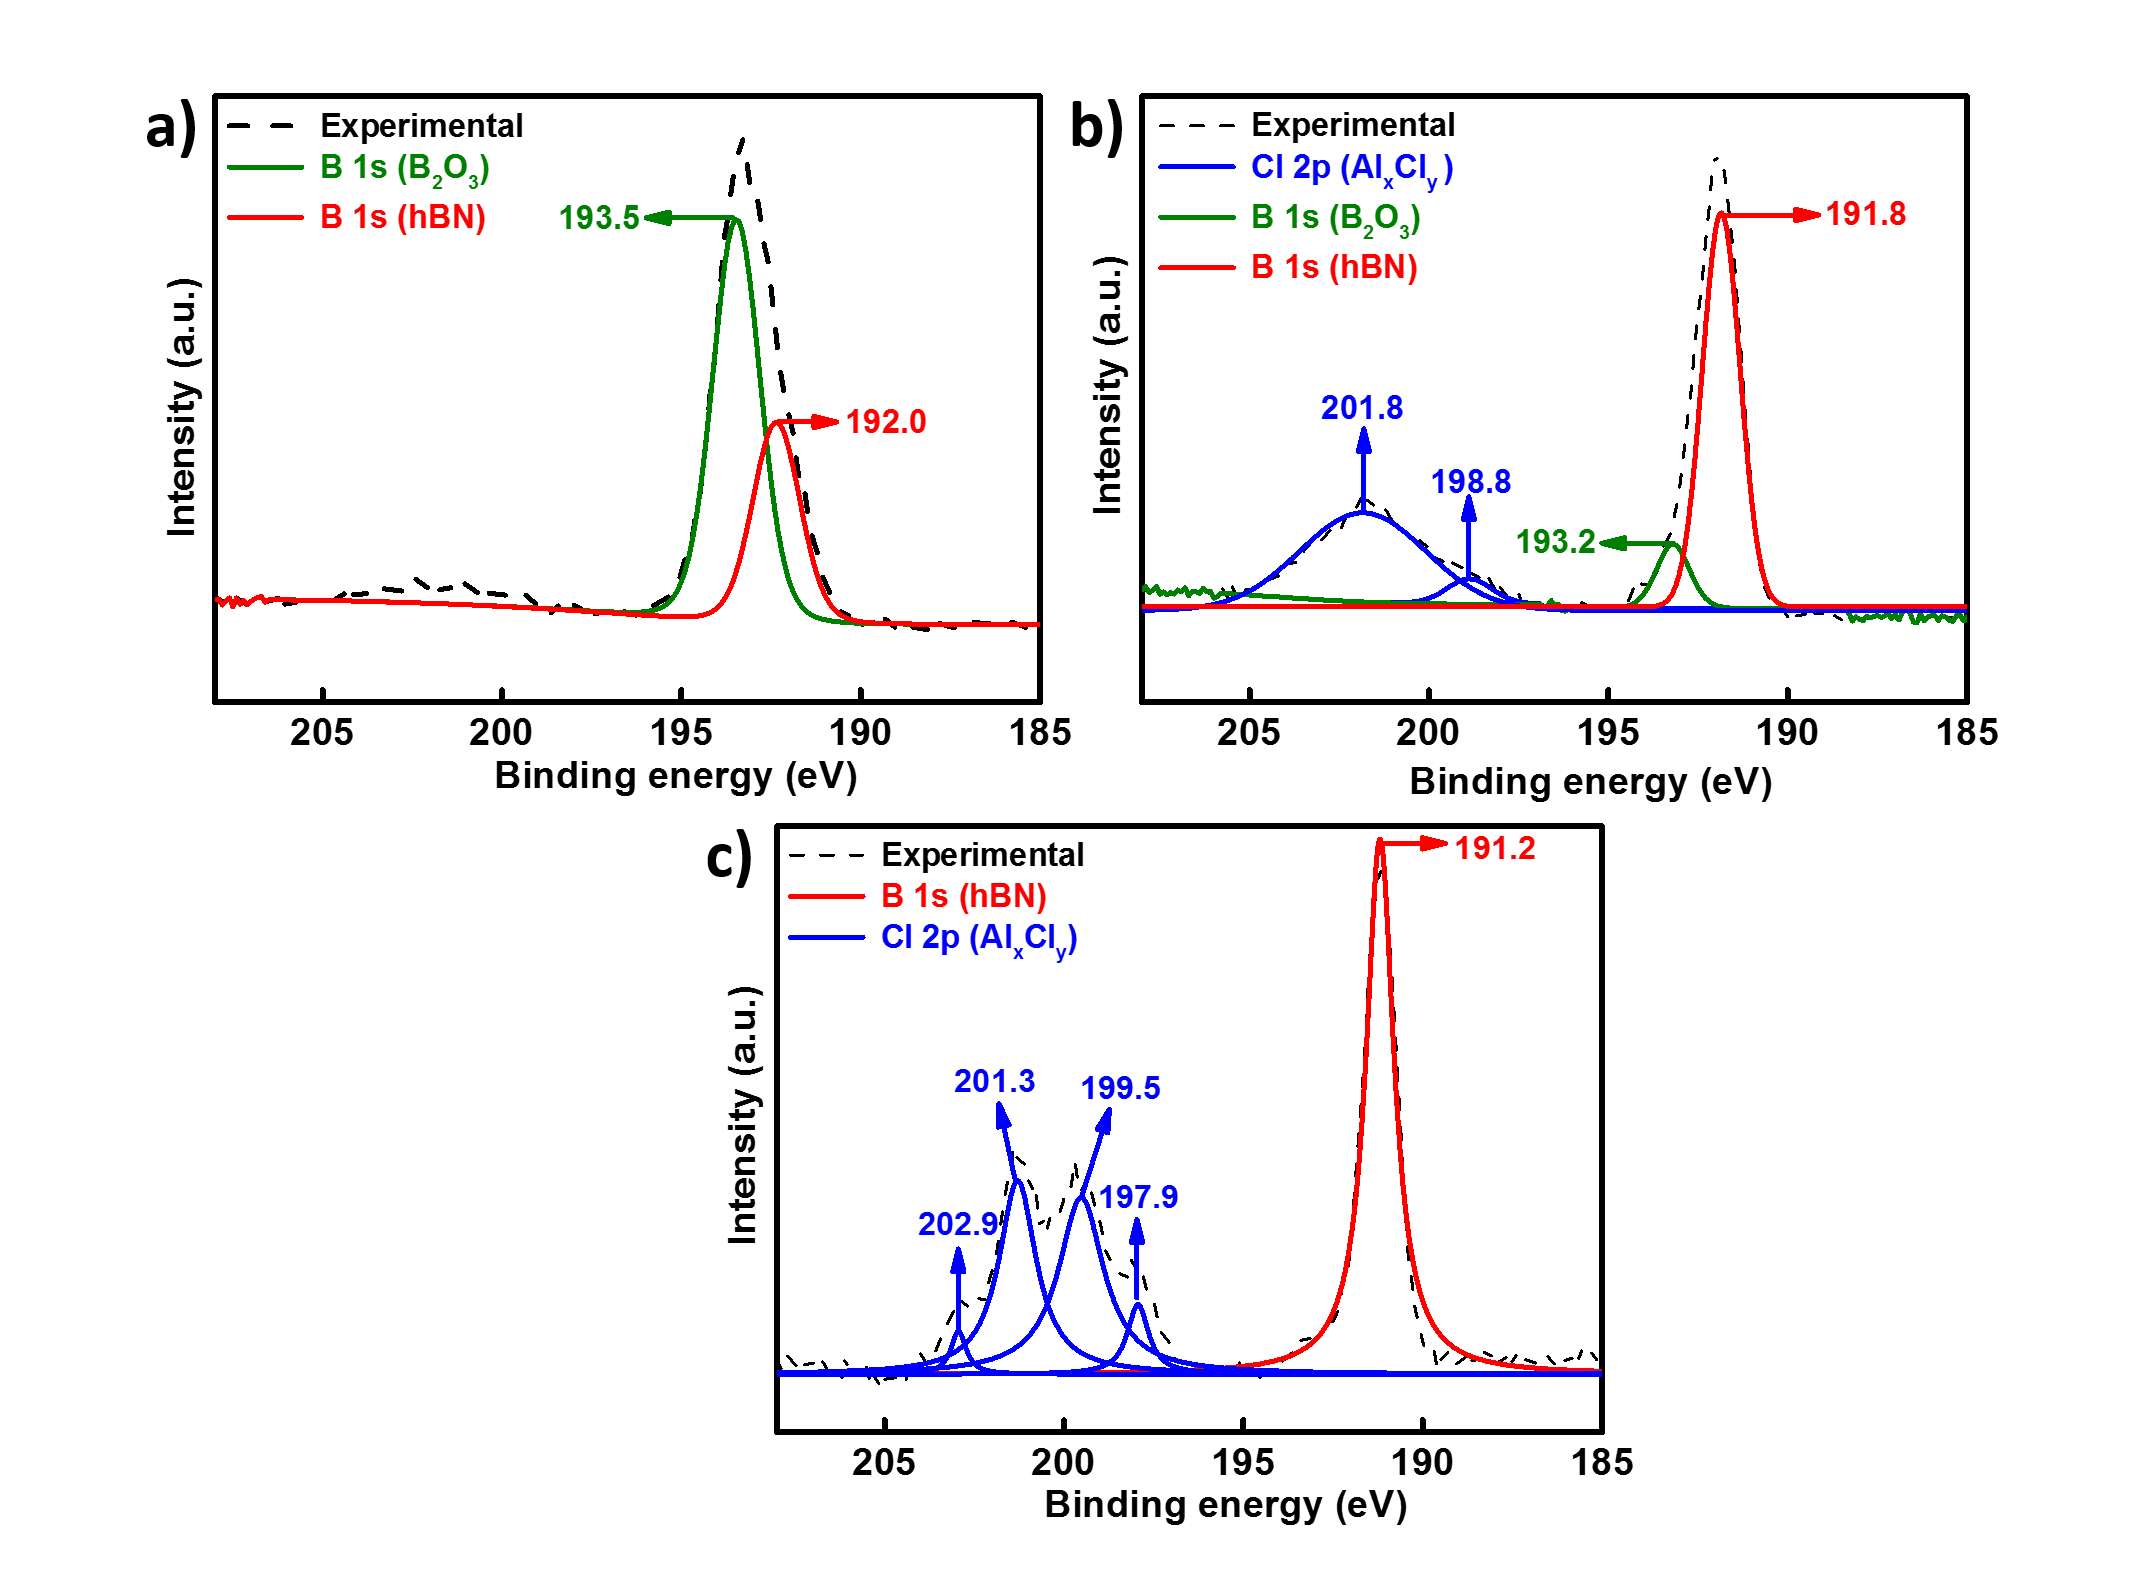
\includegraphics[width=\textwidth]{Figures/BOhBN/oldhBNXPS}
\caption{XPS spectra of a a) pristine, b) charged and c) discharges old hBN cathodes after 30 cycles.}
\label{Figures/BOhBN:oldhBNXPS}
\end{figure}

To examine the changes taking place in the old hBN cathode during charge/discharge cycles, \textit{ex-situ} X-ray photoelectron spectroscopy (XPS) was carried out. The high resolution spectra displaying the binding energies of B 1s and Cl 2p orbitals is shown in Figure \ref{Figures/BOhBN:oldhBNXPS}a-c). The spectra reveal the presence of B and Cl elements for a pristine (Figure \ref{Figures/BOhBN:oldhBNXPS}a) charged (Figure \ref{Figures/BOhBN:oldhBNXPS}b) and discharged (Figure \ref{Figures/BOhBN:oldhBNXPS}c) cathode. Since the pristine electrode was not in contact with the electrolyte, Cl 2p binding energy was absent and the spectra displayed binding energies for boron only. The presence of Cl in the charged and discharged cathodes was mainly derived from the expected intercalation of chloroaluminates into the hBN layers. It can been seen from Figure \ref{Figures/BOhBN:oldhBNXPS}a-c) that the binding energy of B 1s includes a pair of peaks at 193.5 and 192.0 eV before test, which are attributed to B-O (from \ce{B2O3}) and B-N bonds (from hBN) respectively. After charging to 2.35 V, the peak area of the B-O bond significantly decreases. B-N bond from hBN becomes much more dominant. Interestingly, after discharging to 0.3 V, the B-O bond completely disappears as shown in Figure \ref{Figures/BOhBN:oldhBNXPS}c. Binding energy at 191.2 eV was attributed to a B-N bond. Curve fitting for Cl 2p orbital in the charged cathode was problematic. Two broad peaks were fitted into the one broad experimental peak. However, the peak was deconvoluted into 4 peaks at 202.9, 201.3, 199.5 and 197.9 eV after complete discharge. The binding energies (charged cathode) at 193.2 and 191.8 eV are again attributed to B-O from \ce{B2O3} and B-N from hBN respectively. After complete discharge, the B-O bond's binding energy is completely eliminated and only B-N bond remains.

\begin{figure}[tbh!]
\centering
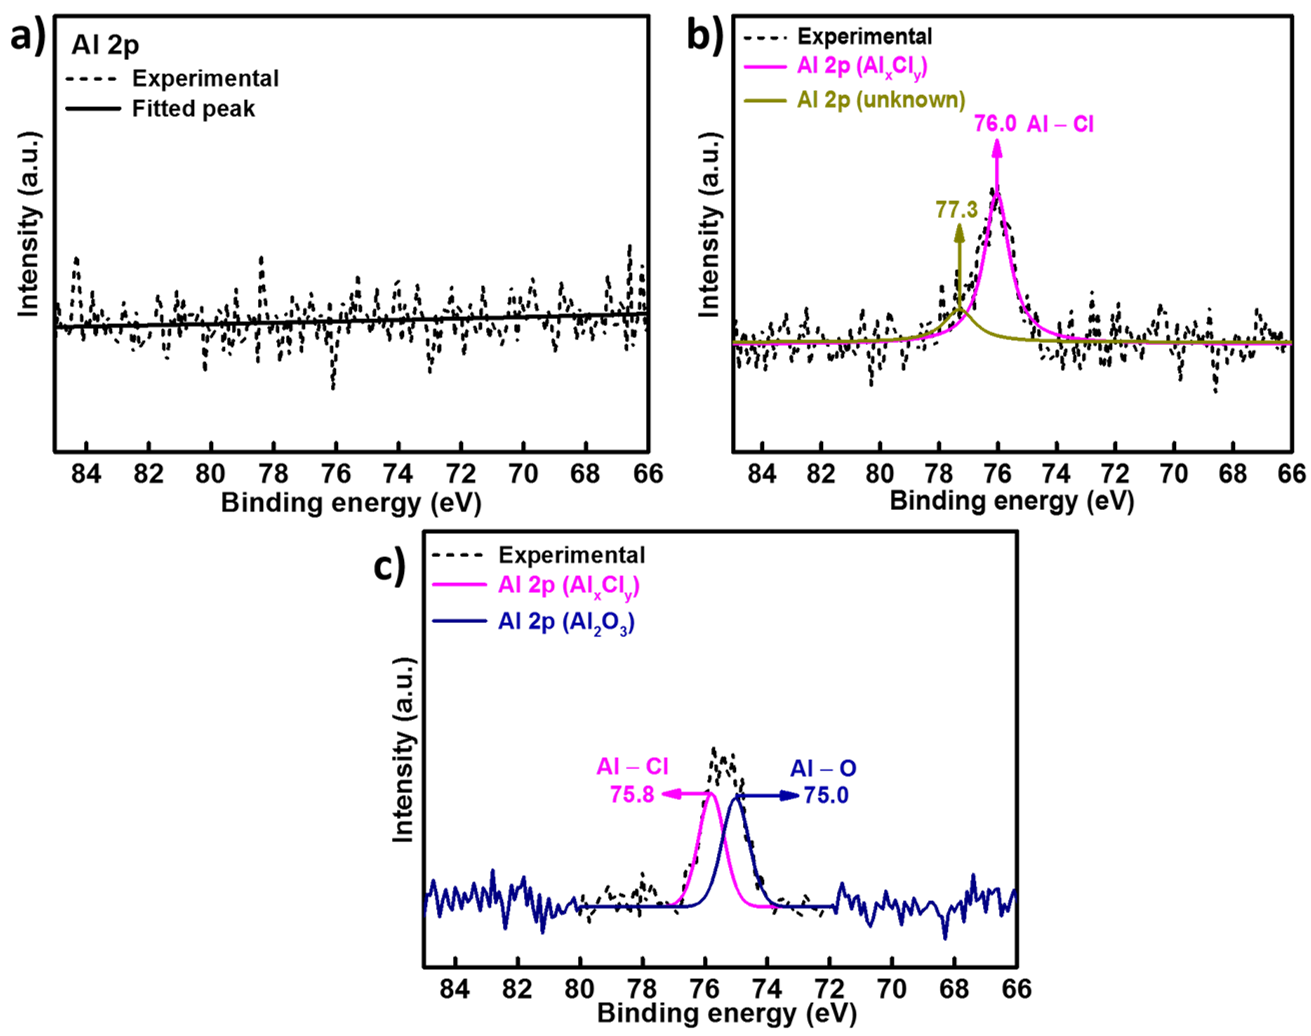
\includegraphics[width=\textwidth]{Figures/BOhBN/hBNAlXPS}
\caption{Honeycomb lattice of a) natural graphite and b) hexagonal boron nitride. Both structures display an interlayer distance of 3.3\AA.}
\label{Figures/BOhBN:hBNAlXPS}
\end{figure}

XPS spectra of Al 2p orbital showed a variation in its binding energies during charge and discharge. During cell charging (Figure \ref{Figures/BOhBN:hBNAlXPS}b), the Al 2p peak deconvolutes into two binding energies at 76.0 and 77.3 eV. The peak at 76.0 eV was attributed to an Al-Cl bond from the chloroaluminates (\ce{AlxCly}). After complete discharge (Figure \ref{Figures/BOhBN:hBNAlXPS}c), the peak shifts to lower binding energies. Experimental curve fitting suggested two binding energies at 75.0 and 75.8 eV. The binding energy at 75.0 eV was attributed to an Al-O bond. It was noted that the binding energy of Al 2p in the oxidised state is 75 eV, which is very close to a typical Al-O bond in \ce{Al2O3} at 74.5 eV \cite{}. This indicated formation of \ce{Al2O3} during discharge. The binding energy at 75.8 eV corresponds to chloroaluminates. It is known that if the electronegativity of the doping element is higher than Al, the electron density around Al decreases and its binding energy increases. Chlorine has a higher electronegativity than oxygen, therefore the peak at higher binding energy in Figure \ref{Figures/BOhBN:hBNAlXPS}c is attributed to \ce{AlxCly} and the lower energy corresponds to \ce{Al2O3}. Since the pristine cathode dis not come in contact with the electrolyte, no peak was observed in Figure \ref{Figures/BOhBN:hBNAlXPS}a for Al. \\*

\begin{figure}[tbh!]
\centering
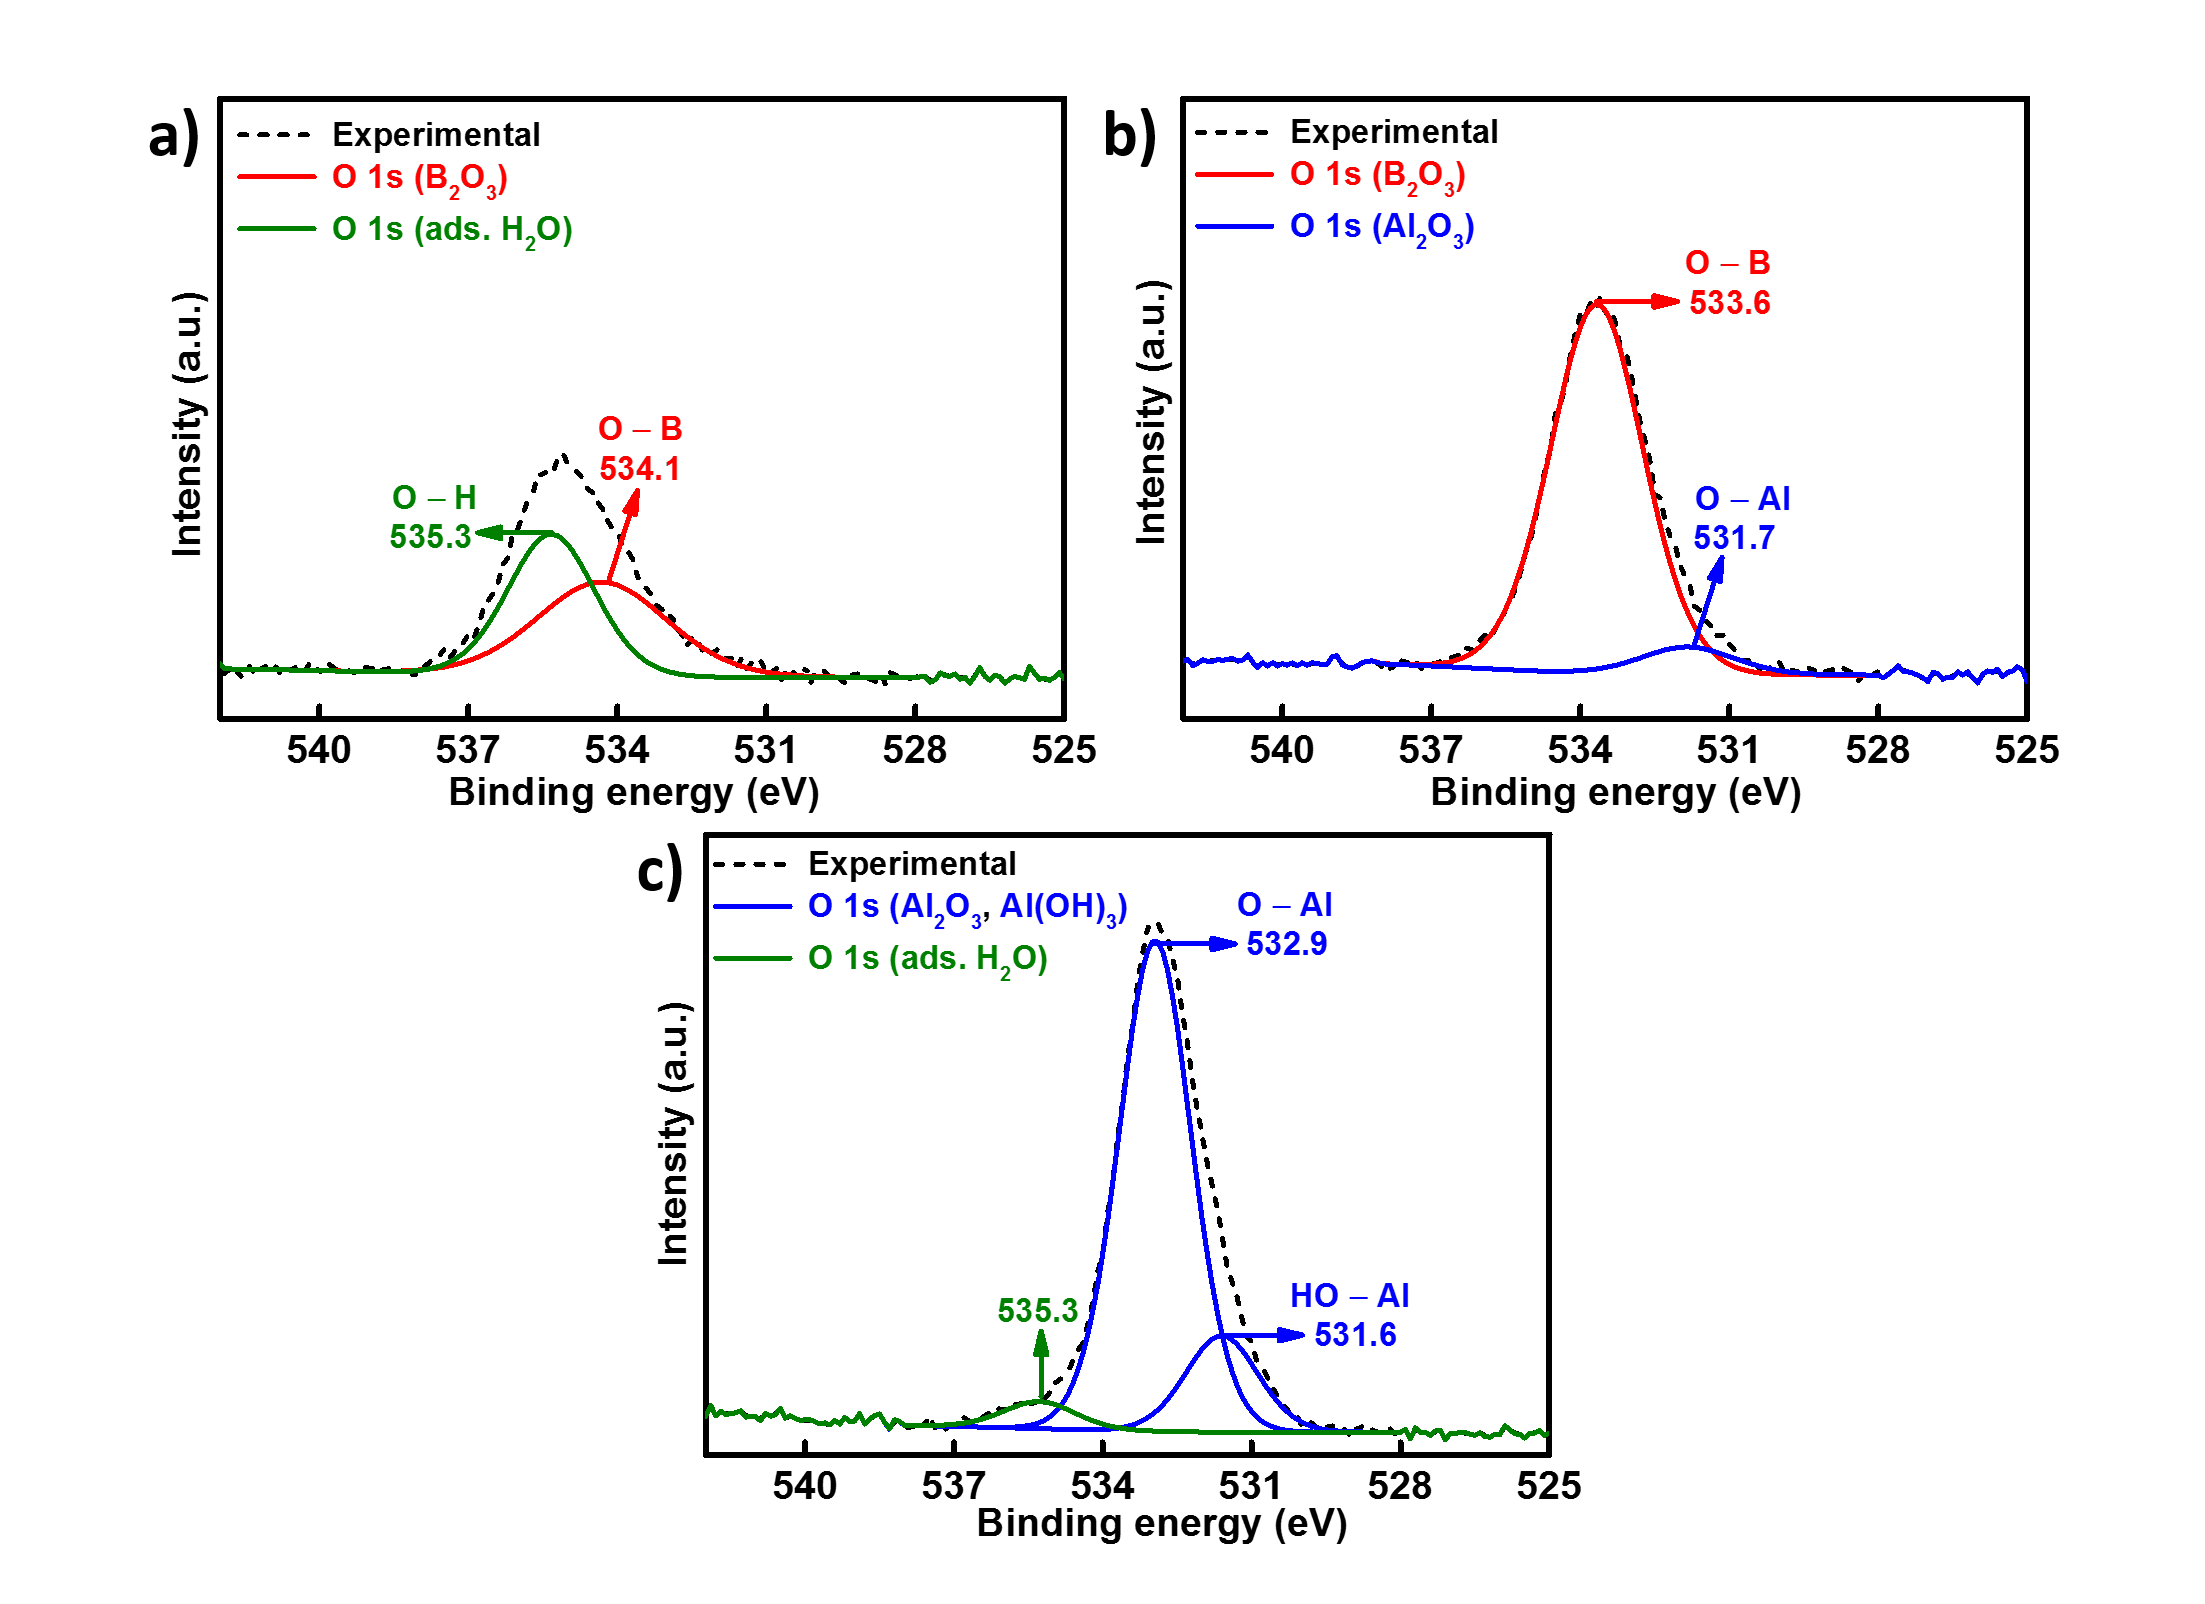
\includegraphics[width=\textwidth]{Figures/BOhBN/hBNOXPS}
\caption{Honeycomb lattice of a) natural graphite and b) hexagonal boron nitride. Both structures display an interlayer distance of 3.3\AA.}
\label{Figures/BOhBN:hBNOXPS}
\end{figure}

Figure \ref{Figures/BOhBN:hBNOXPS}a-c shows the high resolution O 1s spectra of the pristine (Figure \ref{Figures/BOhBN:hBNOXPS}a), charged (Figure \ref{Figures/BOhBN:hBNOXPS}b) and discharged (Figure \ref{Figures/BOhBN:hBNOXPS}c) cathodes made from the old hBN sample. The O 1s core level spectrum for pristine hBN (Figure \ref{Figures/BOhBN:hBNOXPS}a) was split into two peaks that corresponded to an O-H bond at 535.3 eV. This binding energy was attributed to adsorbed moisture (\ce{H2O}) from the environment. The peak at 534.1 eV was attributed to an O-B bond, which confirmed the presence of \ce{B2O3} in the old hBN sample. In the charged cathode, the major contribution of oxygen comes from \ce{B2O3} at 533.6 eV and the remaining from an O-Al bond with a peak at 531.7 eV, suggesting presence of \ce{Al2O3}.  Figure \ref{Figures/BOhBN:hBNOXPS}c shows the spectrum after complete discharge. The peak obtained was deconvoluted into three binding energies at 535.3, 532.9 and 531.6 eV, corresponding to an O-H bond from adsorbed moisture, O-Al and OH-Al bonds from \ce{Al2O3} and possible formation of \ce{Al(OH)3} respectively \cite{}. Following points were concluded from the XPS analysis:
\begin{itemize}
    \item \ce{B2O3} was present in significant amounts in the old hBN sample. However, it disappears completely after discharge. This might suggest the possibility of a conversion reaction where \ce{B2O3} is being converted into something else during discharge.  
    \item \ce{Al2O3} was formed after complete discharge. AL-Cl bonds were present in both charged and discharged electrodes. Even if deintercalation of ions took place during discharge, not all ions came out and a few \ce{AlCl4^-} ions remained in between the layers. However, an Al-Cl bond might also be a result of electrolyte residue on the cathode. 
\end{itemize}

It was assumed that \ce{B2O3} oxidised the \ce{AlCl4^-} ions to \ce{Al2O3} and itself reduced to elemental boron. However, during charge, elemental B was oxidised to \ce{B2O3} and \ce{Al2O3} was reduced back to \ce{AlCl4^-} ions. The conversion reaction in the form of an equation is mentioned below: 

\begin{equation}
    0.5\ce{B2O3 + AlCl3 + 3e-} \longrightarrow \ce{B + 0.5Al2O3 + 3Cl-}
\end{equation}

\begin{figure}[tbh!]
\centering
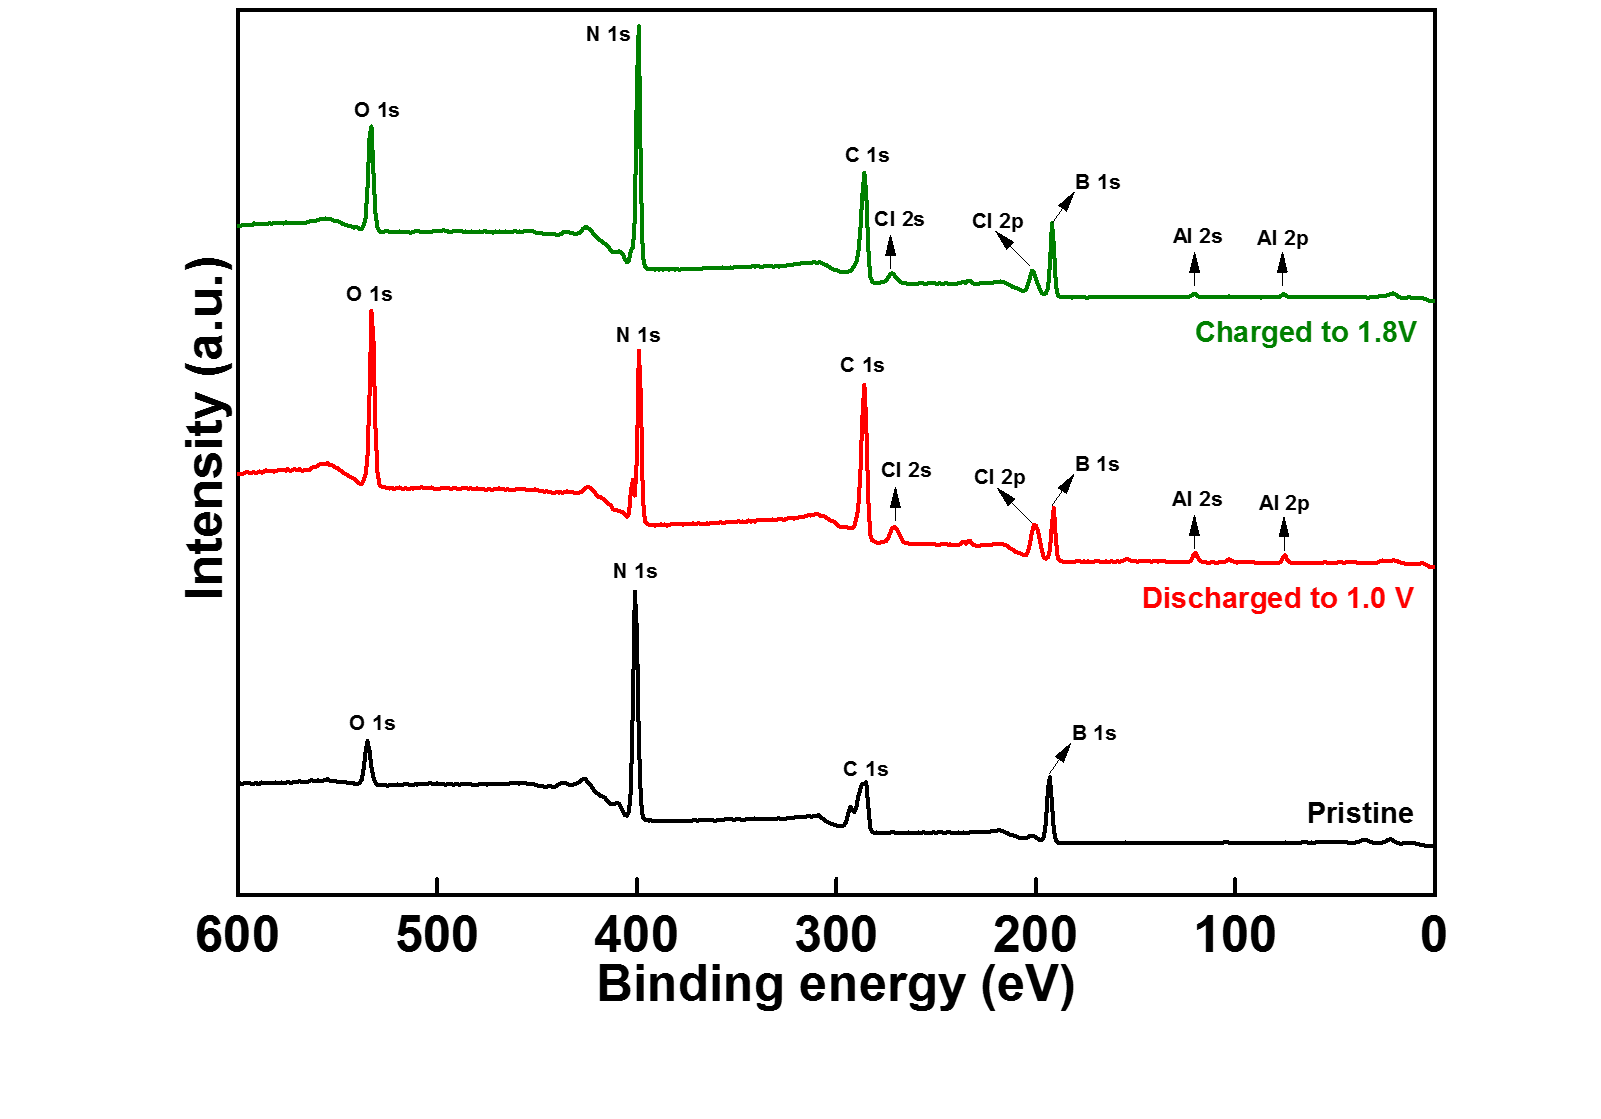
\includegraphics[width=\textwidth]{Figures/BOhBN/hBNXPS}
\caption{A wide scan spectrum of pristine (in black), discharged (in red) and charged (in green) hBN (old) cathode. Figure shows the survey spectra with peaks corresponding to aluminum and chlorine observed in the charged and discharged cathodes. Intensity of Al 2p and Cl 2p is higher in discharged cathode.}
\label{Figures/BOhBN:hBNXPS}
\end{figure}

It was important to find out if hBN played any role in this conversion reaction. hBN has a long-range order in its crystal lattice, while \ce{B2O3} has an amorphous structure. An XRD analysis of the old hBN sample would reveal if the layered structure of hBN allows any intercalation of chloroaluminates and undergoes structural changes during cycles. \\*


\begin{figure}[tbh!]
\centering
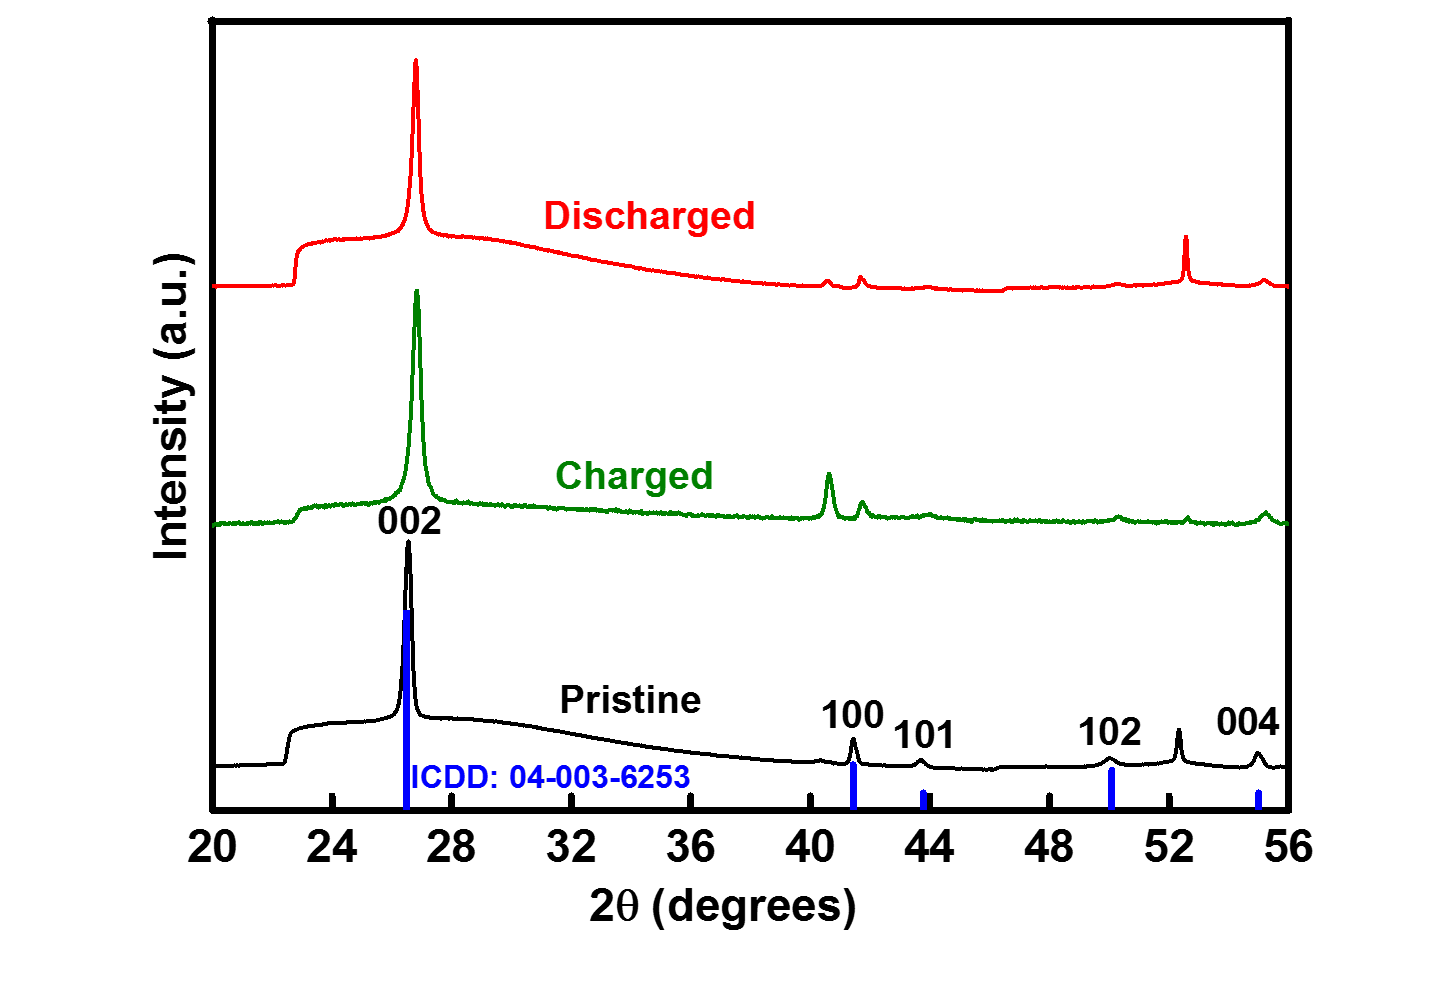
\includegraphics[width=\textwidth]{Figures/BOhBN/hBNXRD2}
\caption{.}
\label{Figures/BOhBN:hBNXRD2}
\end{figure}

In Figure \ref{Figures/BOhBN:hBNXRD2}, X-ray diffraction patterns of pristine (in black), charged (in green) and discharged (in red) cathodes of old hBN is shown. The patterns are in good agreement with the standard ICDD pattern (04-003-6253) and show the existence of hBN with P6/mmc space group. The miller indices (hkl) of all the characteristic peaks are marked as per the standard pattern. Peak at 2$\theta$ value of 26.5$^{\circ}$ confirms the d-spacing of 3.3\AA\, which matches well with the 002 plane of hBN. An additional shoulder that begins at 22$^{\circ}$ suggested presence of amorphous \ce{B2O3}. Interestingly, a new peak was observed at a 2$\theta$ value of 52.36$^{\circ}$. This peak matched with xxx plane of \ce{B2O3} (ICDD:). There was a slight shift observed for some peaks during the charge and discharge process. The peaks at 100 and 101 shift to lower 2$\theta$ values. This indicated an increase in the d-spacing value. The spacing increased from to 2.17 \AA to 2.22\AA for 100 and from 2.06\AA to 2.16\AA for 101 plane after cycles. In an ideal case, when ions intercalate during charging, the d-spacing increases and then when the ions deintercalate during discharging, the d-spacing returns back to its original value \cite{wang_advanced_2017}. In this case however, the d-spacing does not shift back to its original value after discharge. This suggests that the structural changes that take place during cycles in the hBN crystal lattice are permanent in nature. Since hBN is more crystalline in nature and therefore dominates the XRD data, it was difficult to study the patterns obtained from \ce{B2O3}.  \\*

\textit{Ex-situ} SEM experiments were also conducted to determine the structural changes taking place in the old hBN cathode. Figure \ref{Figures/BOhBN:hBNSEM} displays the SEM images of hBN cathode before and after cycles. Although a few sites showed agglomeration after cycles in Figure \ref{Figures/BOhBN:hBNSEM}b and d, it was difficult to make conclusions from these images.

\begin{figure}[tbh!]
\centering
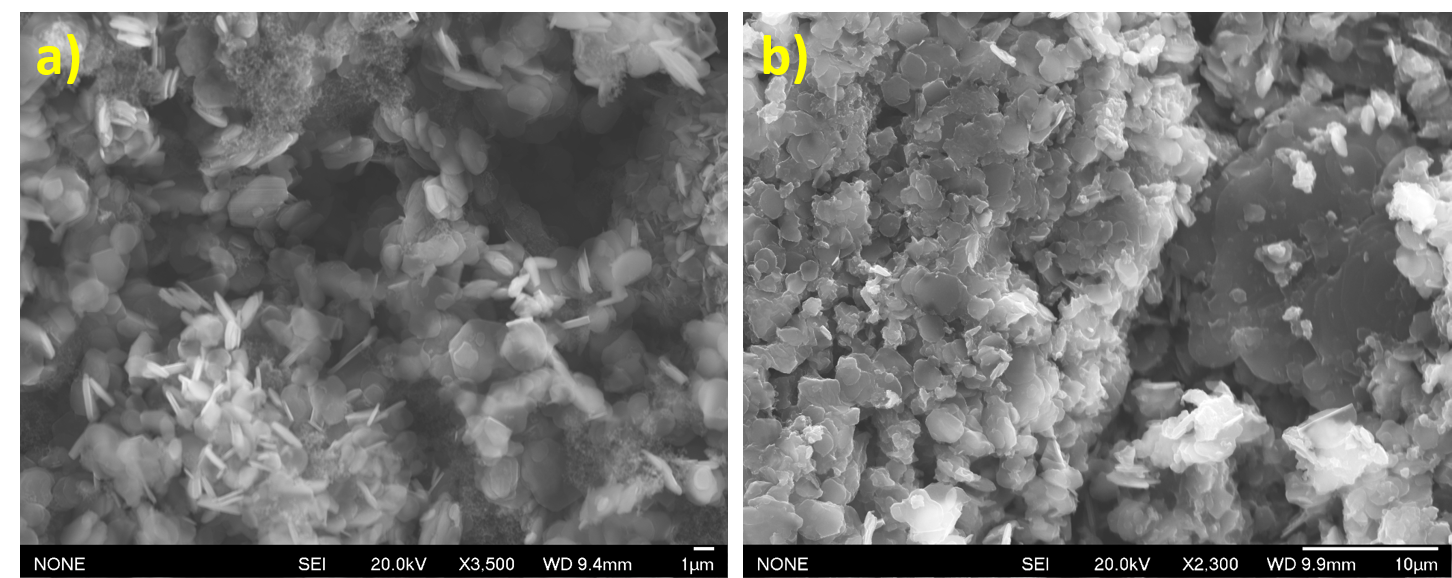
\includegraphics[width=\textwidth]{Figures/BOhBN/hBNSEM}
\caption{SEM images of a), c) pristine hBN. The hexagonal shape of boron nitride is distinctly visible. Figure\ref{Figures/BOhBN:hBNSEM} b and d) suggest that after a few cycles, the particles agglomerate. The particles retain their distinct hexagonal shape.}
\label{Figures/BOhBN:hBNSEM}
\end{figure}



\section*{Pure boric anhydride \ce{B2O3} as an active material}
To find determine how \ce{B2O3} performed as a cathode material in absence of hBN, cells were assembled using \ce{B2O3} as the active material and the results are shown in Figure \ref{Figures/BOhBN:BOCDC}. 

\begin{figure}[tbh!]
\centering
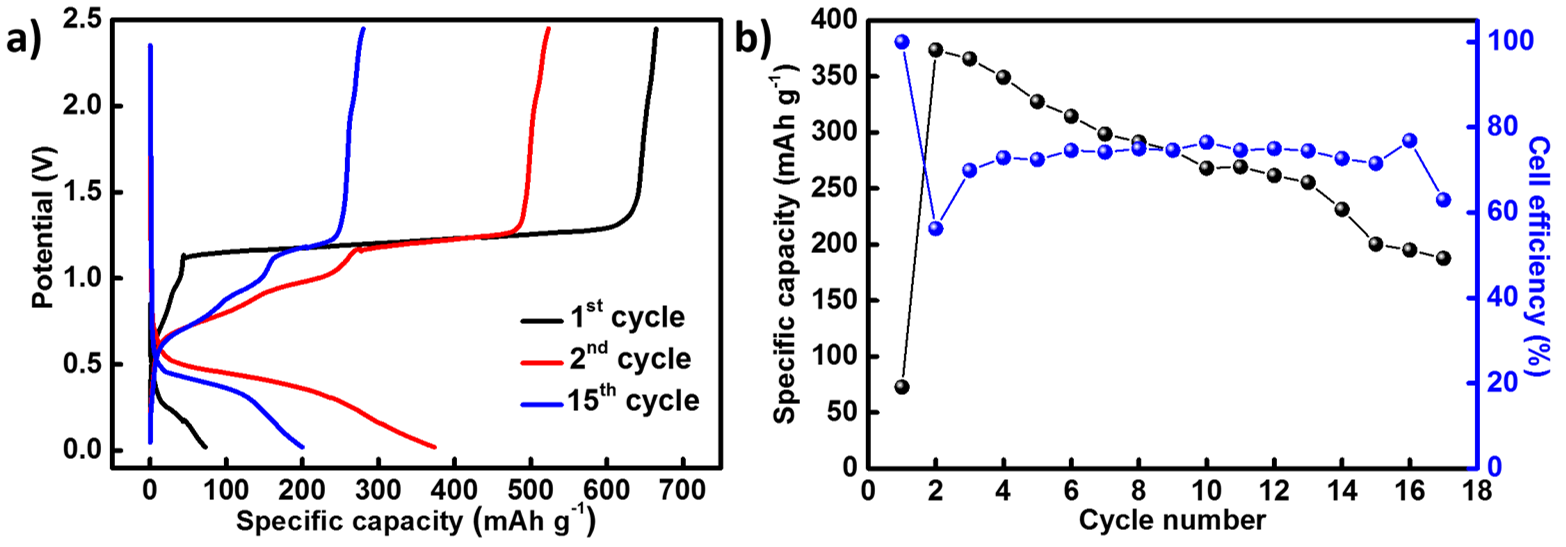
\includegraphics[width=\textwidth]{Figures/BOhBN/BOCDC}
\caption{Charge/discharge profile of pure \ce{B2O3} as the active material in an AIB at the current rate of 50 mA g$^{-1}$. After 15 cycles, the capacity drops by $\sim$50\%. Coulombic efficiency of Al/\ce{B2O3} is low and  stabilises at $\sim$78\%.}
\label{Figures/BOhBN:BOCDC}
\end{figure}

\ce{B2O3} achieved a discharge capacity of 390 mAh g$^{-1}$ in its first cycle, which decreased to 200 mAh g$^{-1}$ in its second cycle and further dropped down to 90 mAh g$^{-1}$ after 15 cycles. Significant amount of capacity fading was observed, although coulombic efficiency of $\sim$ 78\% was maintained. It was possible that hBN provided structural support to \ce{B2O3}, therefore a combination of both was required to store high amounts of charge Figure \ref{Figures/appendix:hBNrepeat}. 

\begin{figure}[tbh!]
\centering
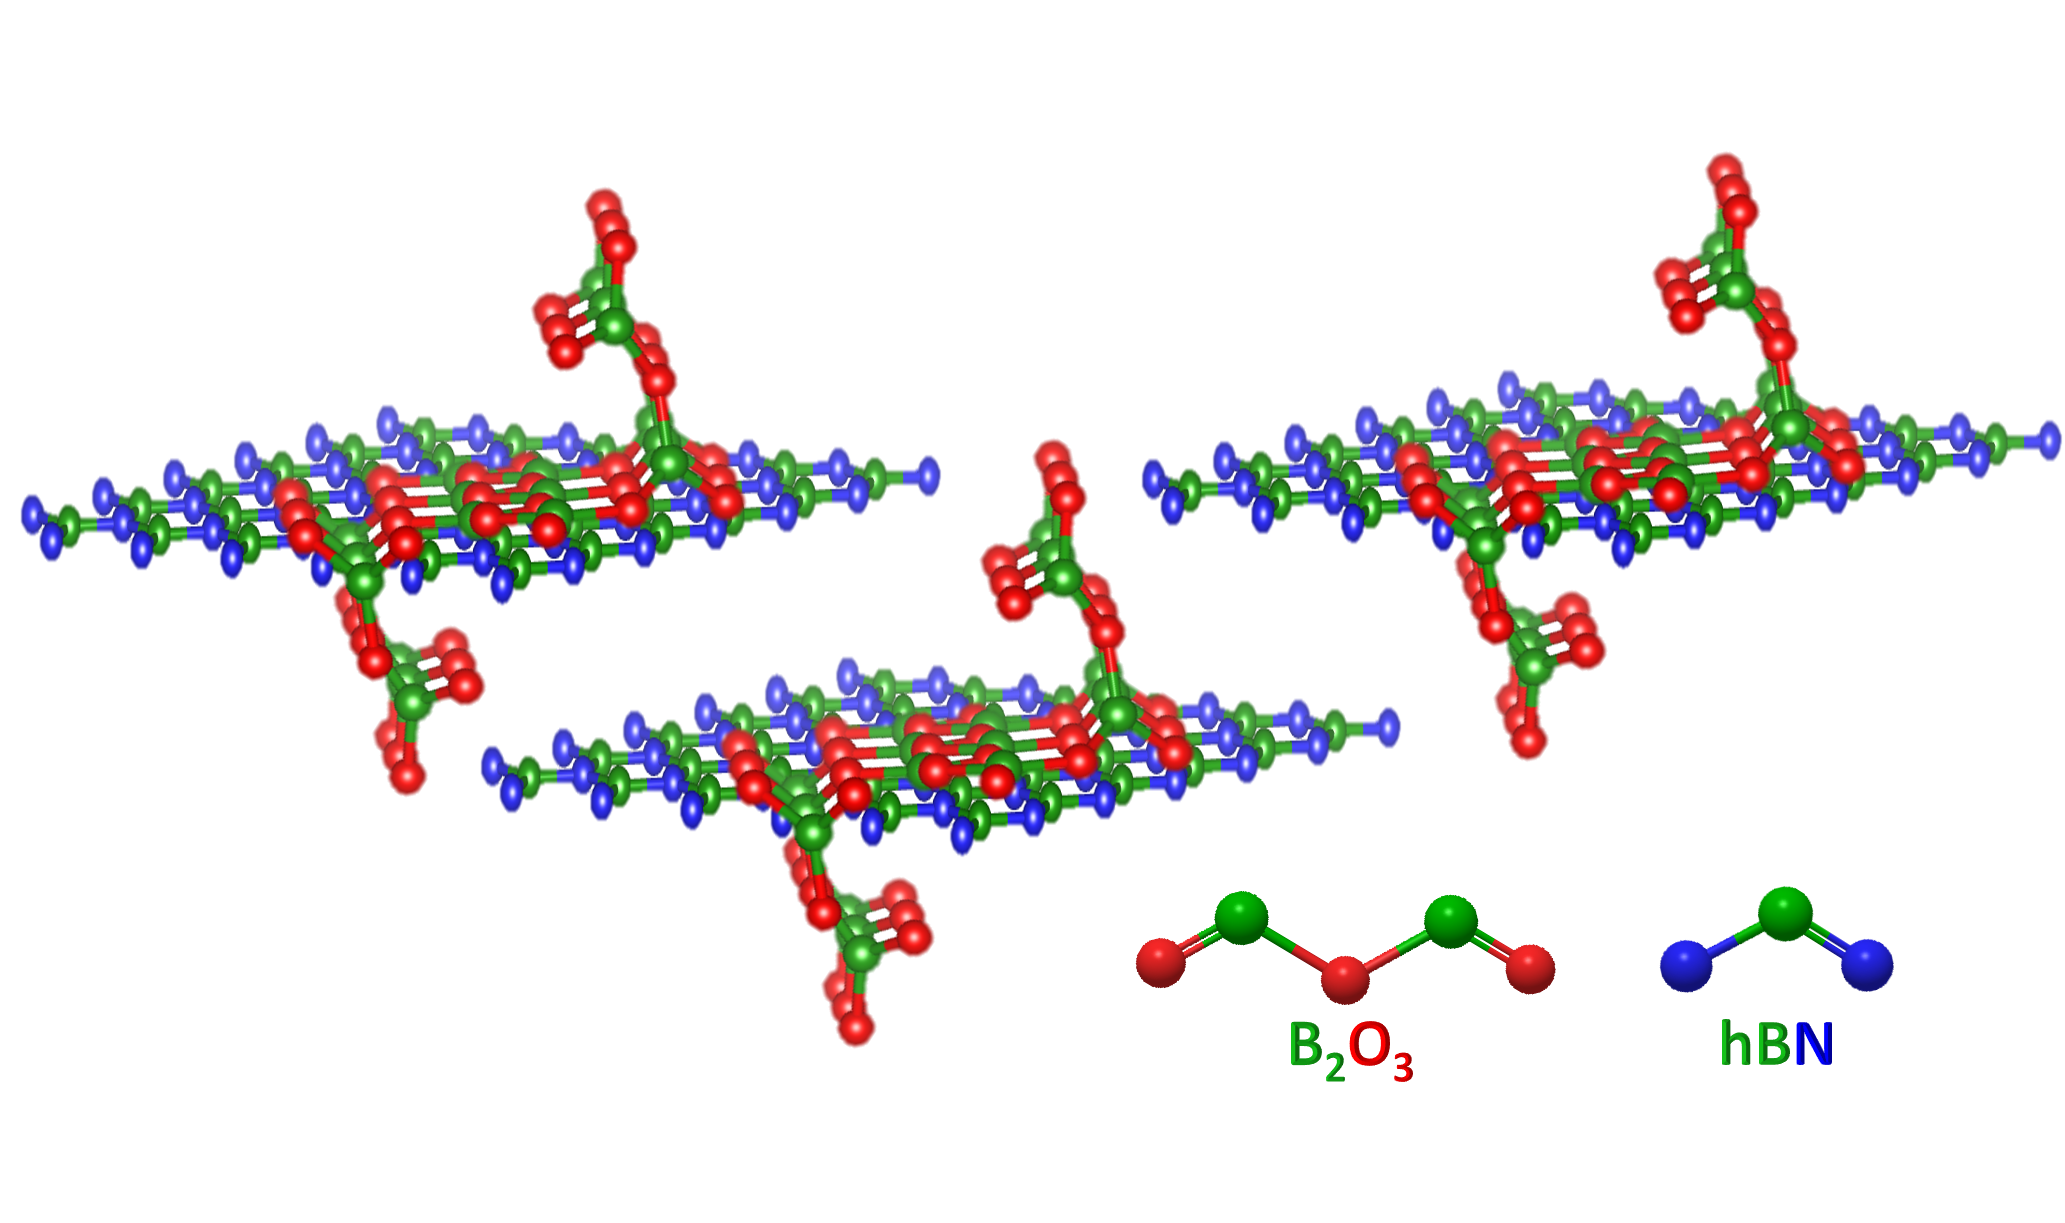
\includegraphics[width=\textwidth]{Figures/BOhBN/BonhBN}
\caption{Schematic showing the layered structure of hBN supporting \ce{B2O3}. During discharge \ce{AlCl3} reacts with \ce{B2O3} resulting in formation of elemental boron and \ce{Al2O3} and free \ce{Cl-} ions. Further analysis is needed to fully understand the role of hBN.}
\label{Figures/BOhBN:BohBN}
\end{figure}

The ratio of hBN  and \ce{B2O3} in the old sample was unknown. For this reason, different weight ratios of hBN and \ce{B2O3} were investigated as cathodes. The ratios and their performance is tabulated below in Table \ref{tabdiffpc}. All cells achieved discharge voltage plateaus at $\sim$ 0.6 V. 50\% hBN/50\%\ce{B2O3} was the best performing cathode amongst all tested ratios. The results for 1:1 hBN/\ce{B2O3} are displayed in Figure \ref{Figures/BOhBN:hBNBO5050}. Since a conversion reaction (Equation 6.1) was taking place during electron transfer, evaluating a combination of other nitrides and oxides was an important part of this chapter. As the optimum ratio obtained for hBN /\ce{B2O3} cathode was 1:1, all new nitrides and oxides were mixed in that same ratio. 

\begin{table}[tbh!]
\centering
\caption{Comparing performance of hBN/\ce{B2O3} cathodes at different weight percentages.} \label{tabdiffpc}
\begin{tabular}{|ccc|}
\hline
\textbf{Weight \% of} & \textbf{Weight \% of} & \textbf{Discharge capacity in 20th cycle} \\
\textbf{hBN} & \textbf{\ce{B2O3}} & \textbf{mAh g$^{-1}$} \\
\hline
\hline
50 & 50 & 120\\
25 & 75 & 22\\
20 & 80 & 48\\
15 & 85 & 48\\
10 & 90 & 68\\
5 & 95 & 171\\
0 & 100 & 104\\
\hline 
\end{tabular}
\end{table}

\begin{figure}[tbh!]
\centering
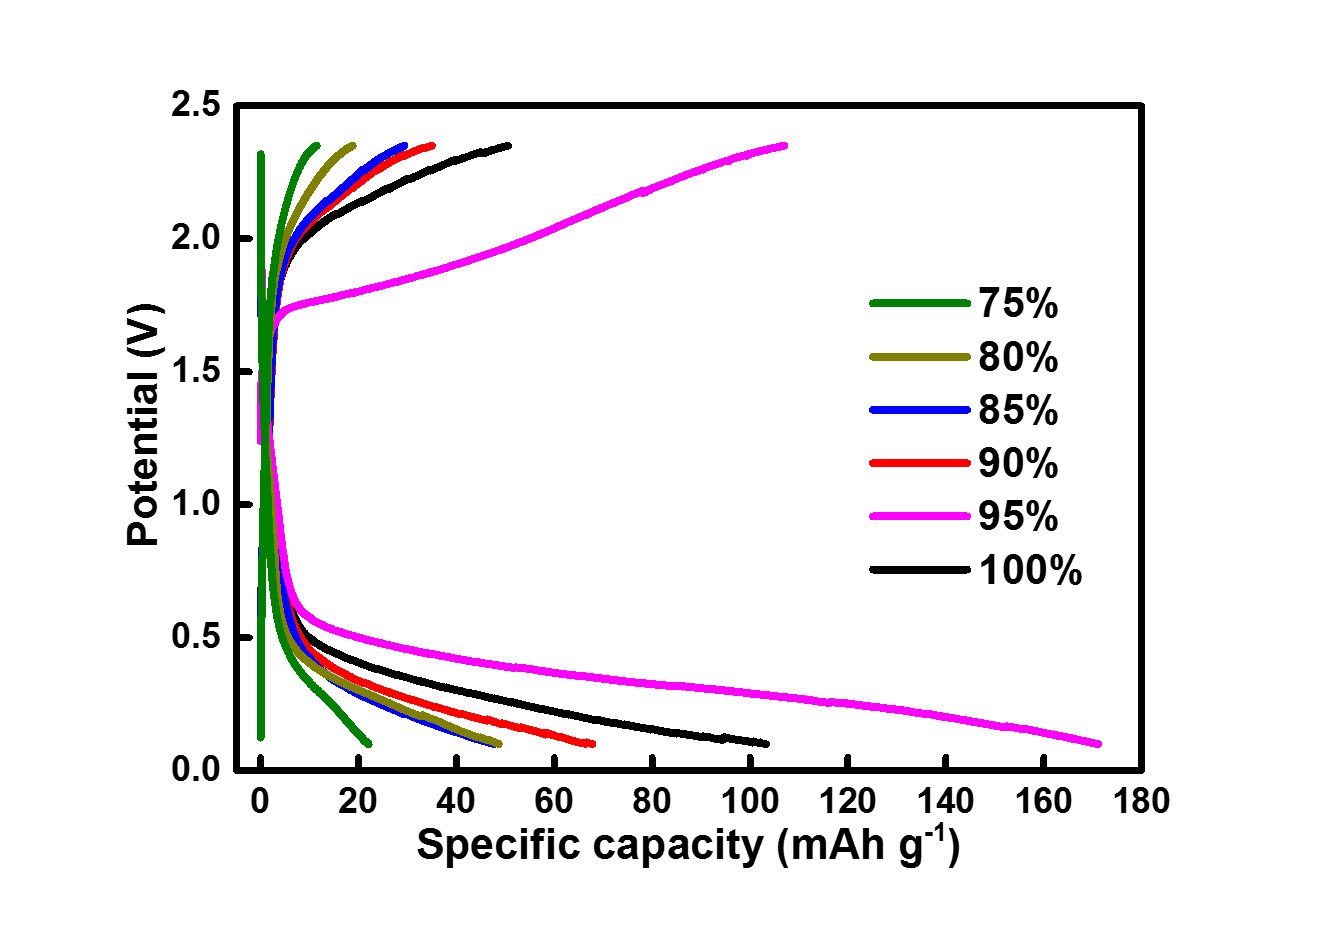
\includegraphics[width=\textwidth]{Figures/BOhBN/hBNBOdifpc}
\caption{Charge/discharge curves of aluminium-ion cells with \ce{B2O3}/hBN as cathode in their 20$^{th}$ cycle. The weight percentage varied from 75\%\ce{B2O3}-25\%hBN to 100\% pure\ce{B2O3}.}
\label{Figures/BOhBN:hBNdifpc}
\end{figure}



\begin{figure}[tbh!]
\centering
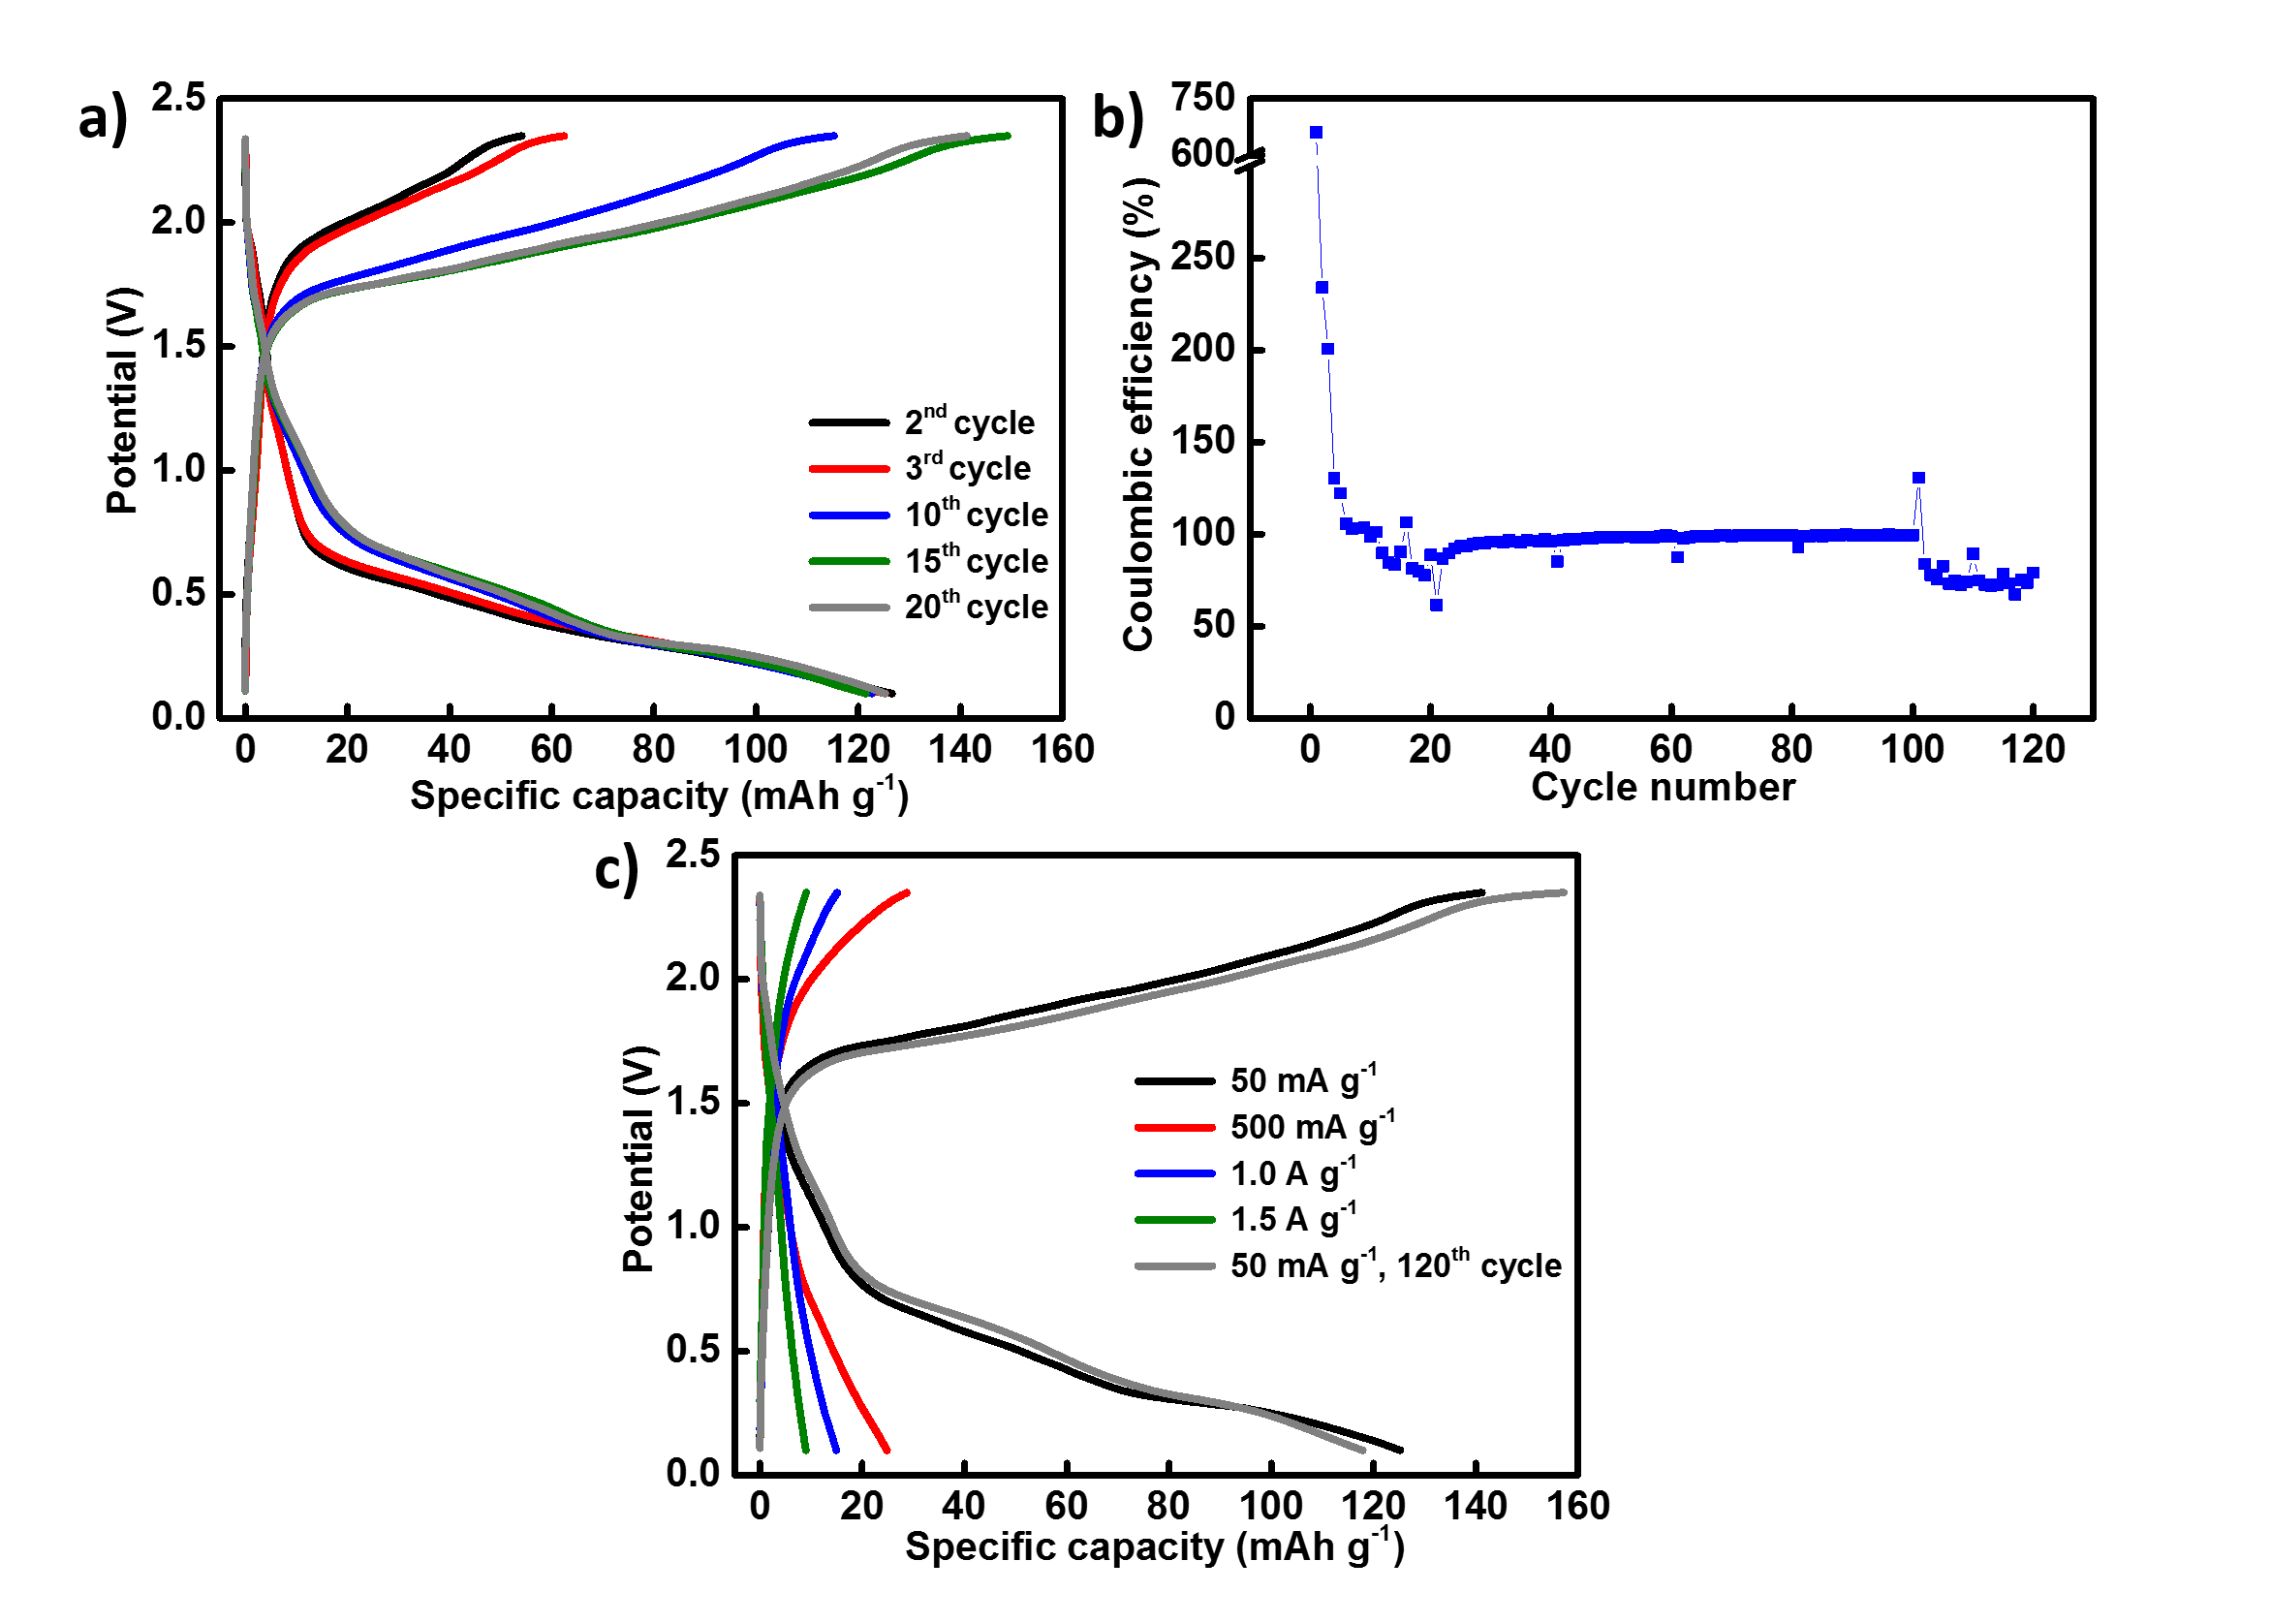
\includegraphics[width=\textwidth]{Figures/BOhBN/hBNBO5050}
\caption{Charge/discharge curves of hBN/ \ce{B2O3} cells a) for the first 20 cycles at a current rate of 50 mA g$^{-1}$, b) coulombic efficiencies and c) long term cell performance at various current densities ranging from 50 mA g$^{-1}$ to 1500 mA g$^{-1}$ .}
\label{Figures/BOhBN:hBNBO5050}
\end{figure}

Other nitrides such as graphitic carbon nitride g-\ce{C3N4}, aluminium nitride (AlN) and silicon nitride (\ce{Si3N4}) were mixed with \ce{B2O3} in a ratio of 1:1 and tested as cathodes. The results are displayed in Figure \ref{Figures/BOhBN:Bonit}. 
\begin{figure}[tbh!]
\centering
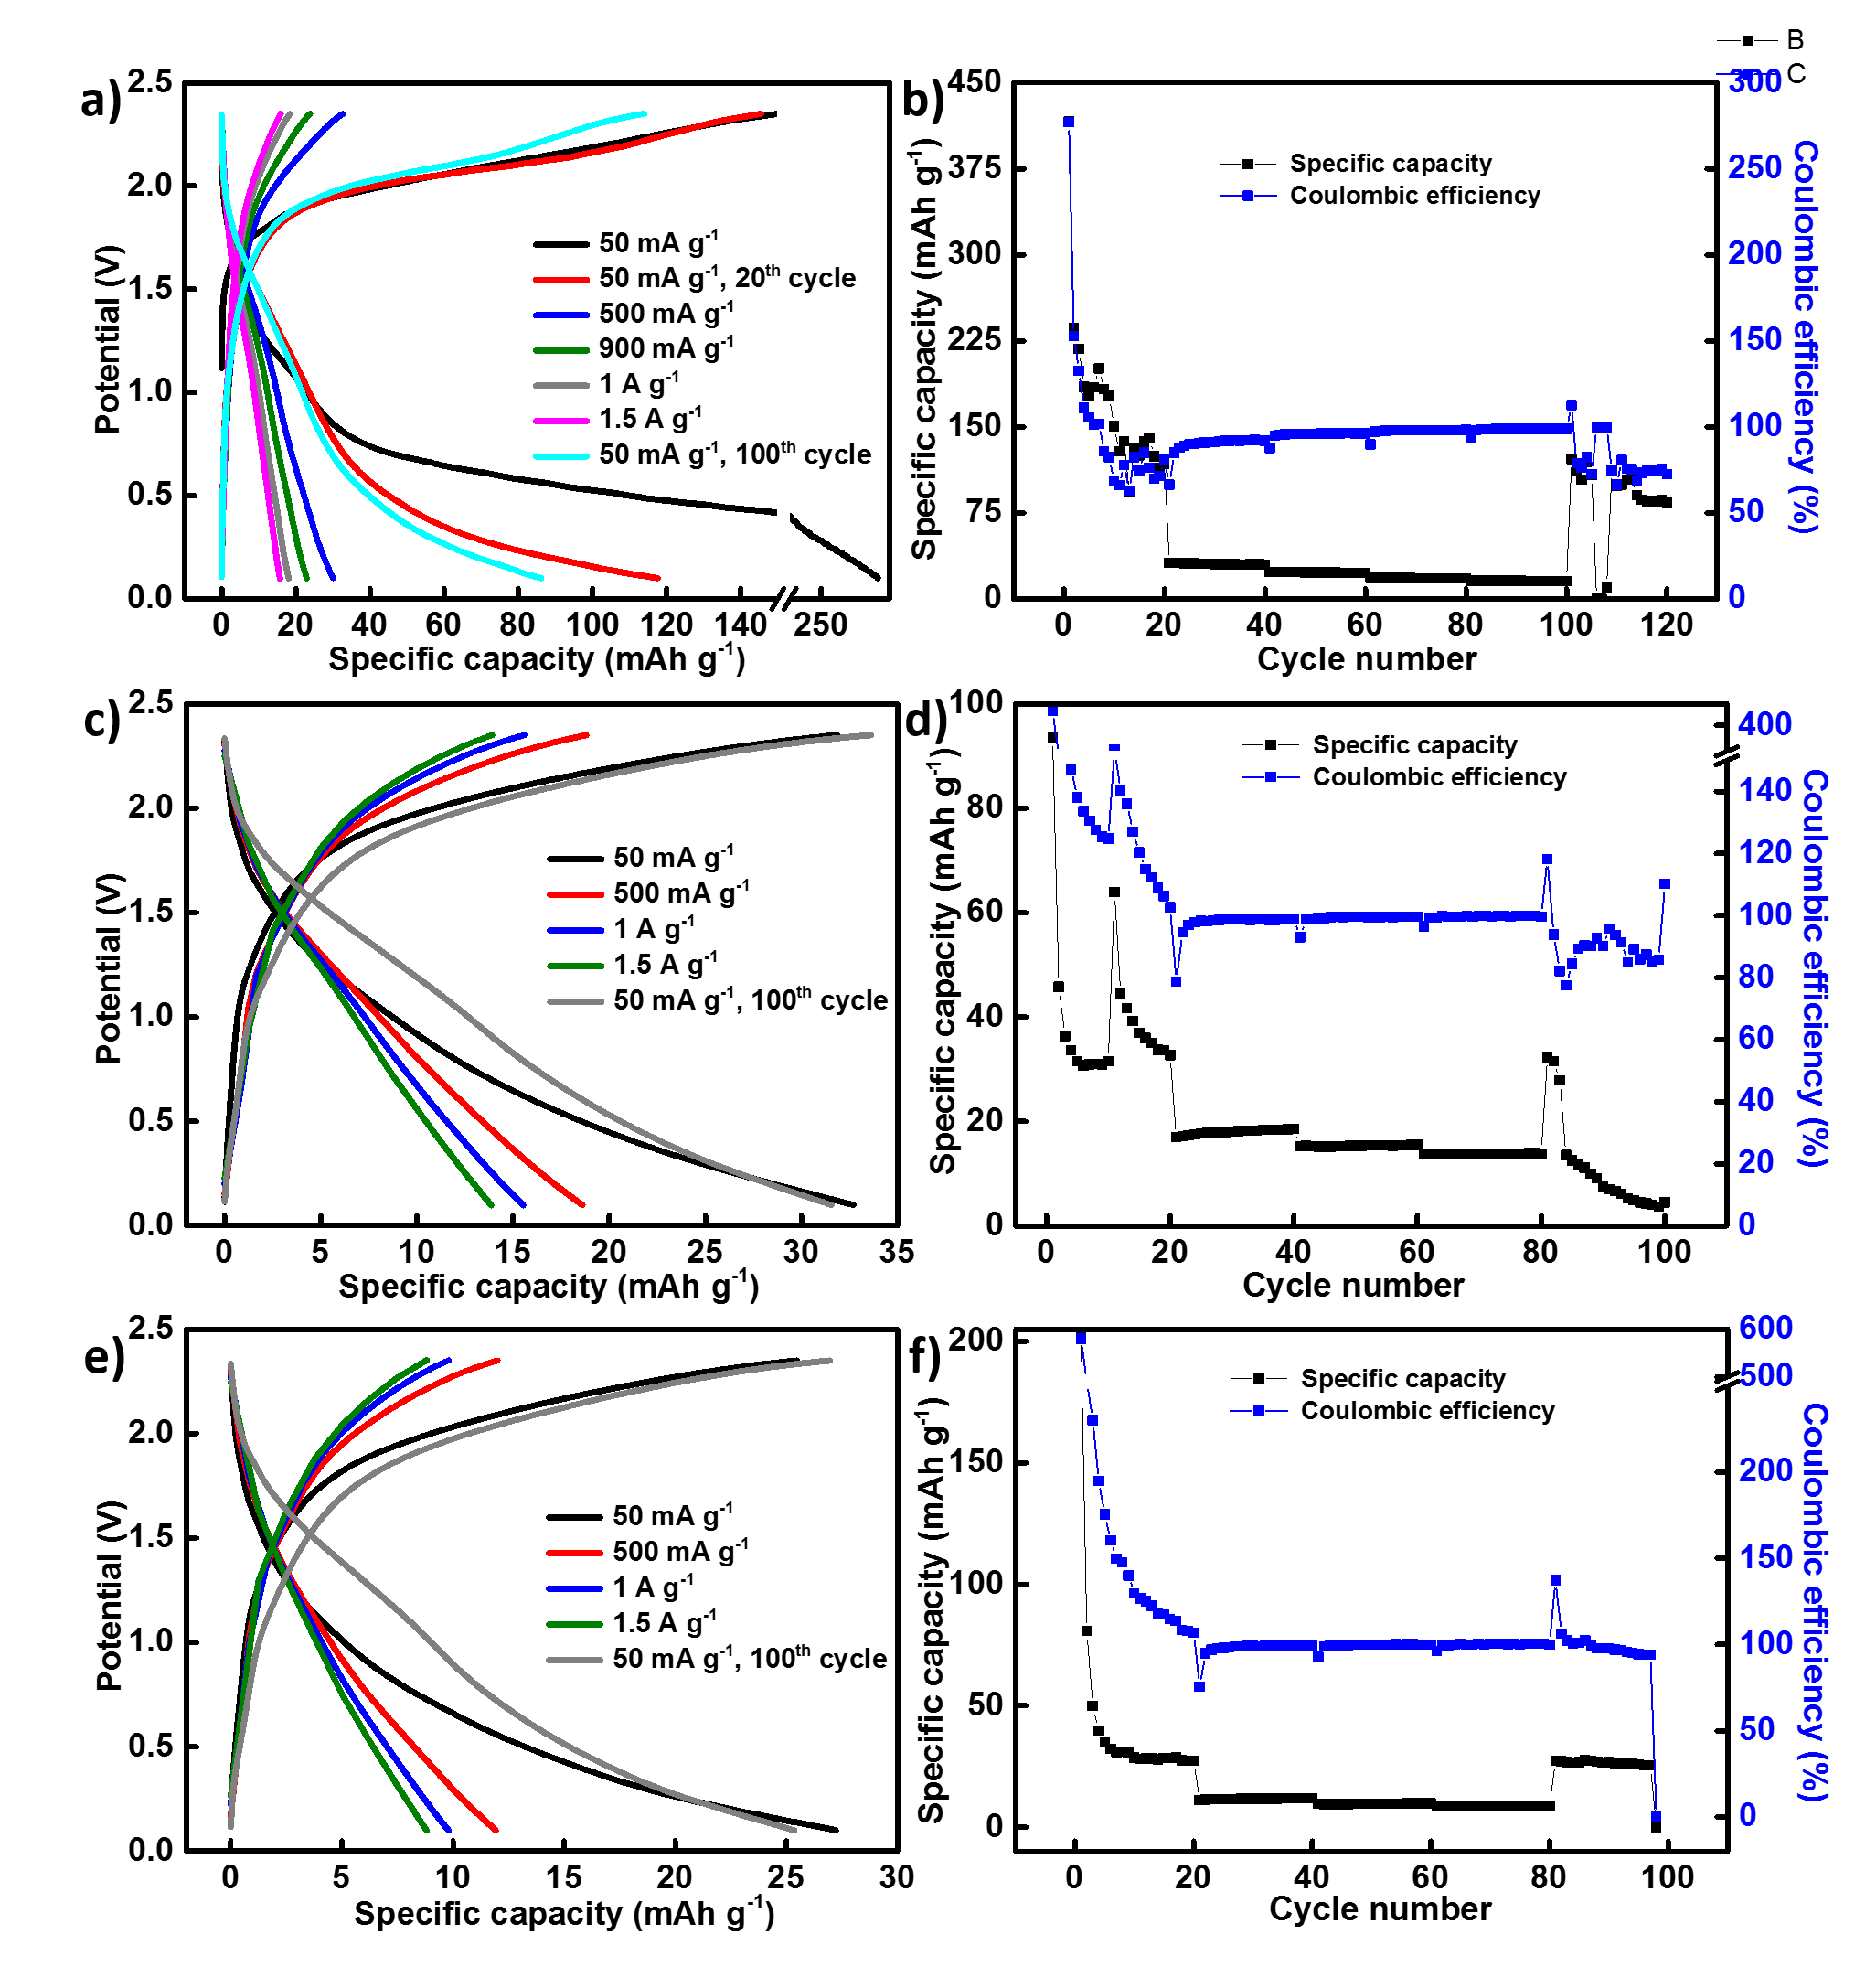
\includegraphics[width=\textwidth]{Figures/BOhBN/Bonit}
\caption{Galvanostatic charge/discharge cycles of cells at different current rates using \ce{B2O3} mixed with other nitrides such as a) \ce{C3N4}, c) AlN and e) \ce{Si3N4} as cathodes. Coulombic efficiencies of b) \ce{B2O3}/\ce{C3N4}, d) \ce{B2O3}/AlN and f) \ce{B2O3}/\ce{Si3N4} cells .}
\label{Figures/BOhBN:Bonit}
\end{figure}

Other oxides such as manganese dioxide (\ce{MnO2}) and titanium dioxide (\ce{TiO2}) were mixed with hBN in a ratio of 1:1 and tested as cathodes for AIBs. The results are displayed in Figure \ref{Figures/BOhBN:BNdifO}.

\begin{figure}[tbh!]
\centering
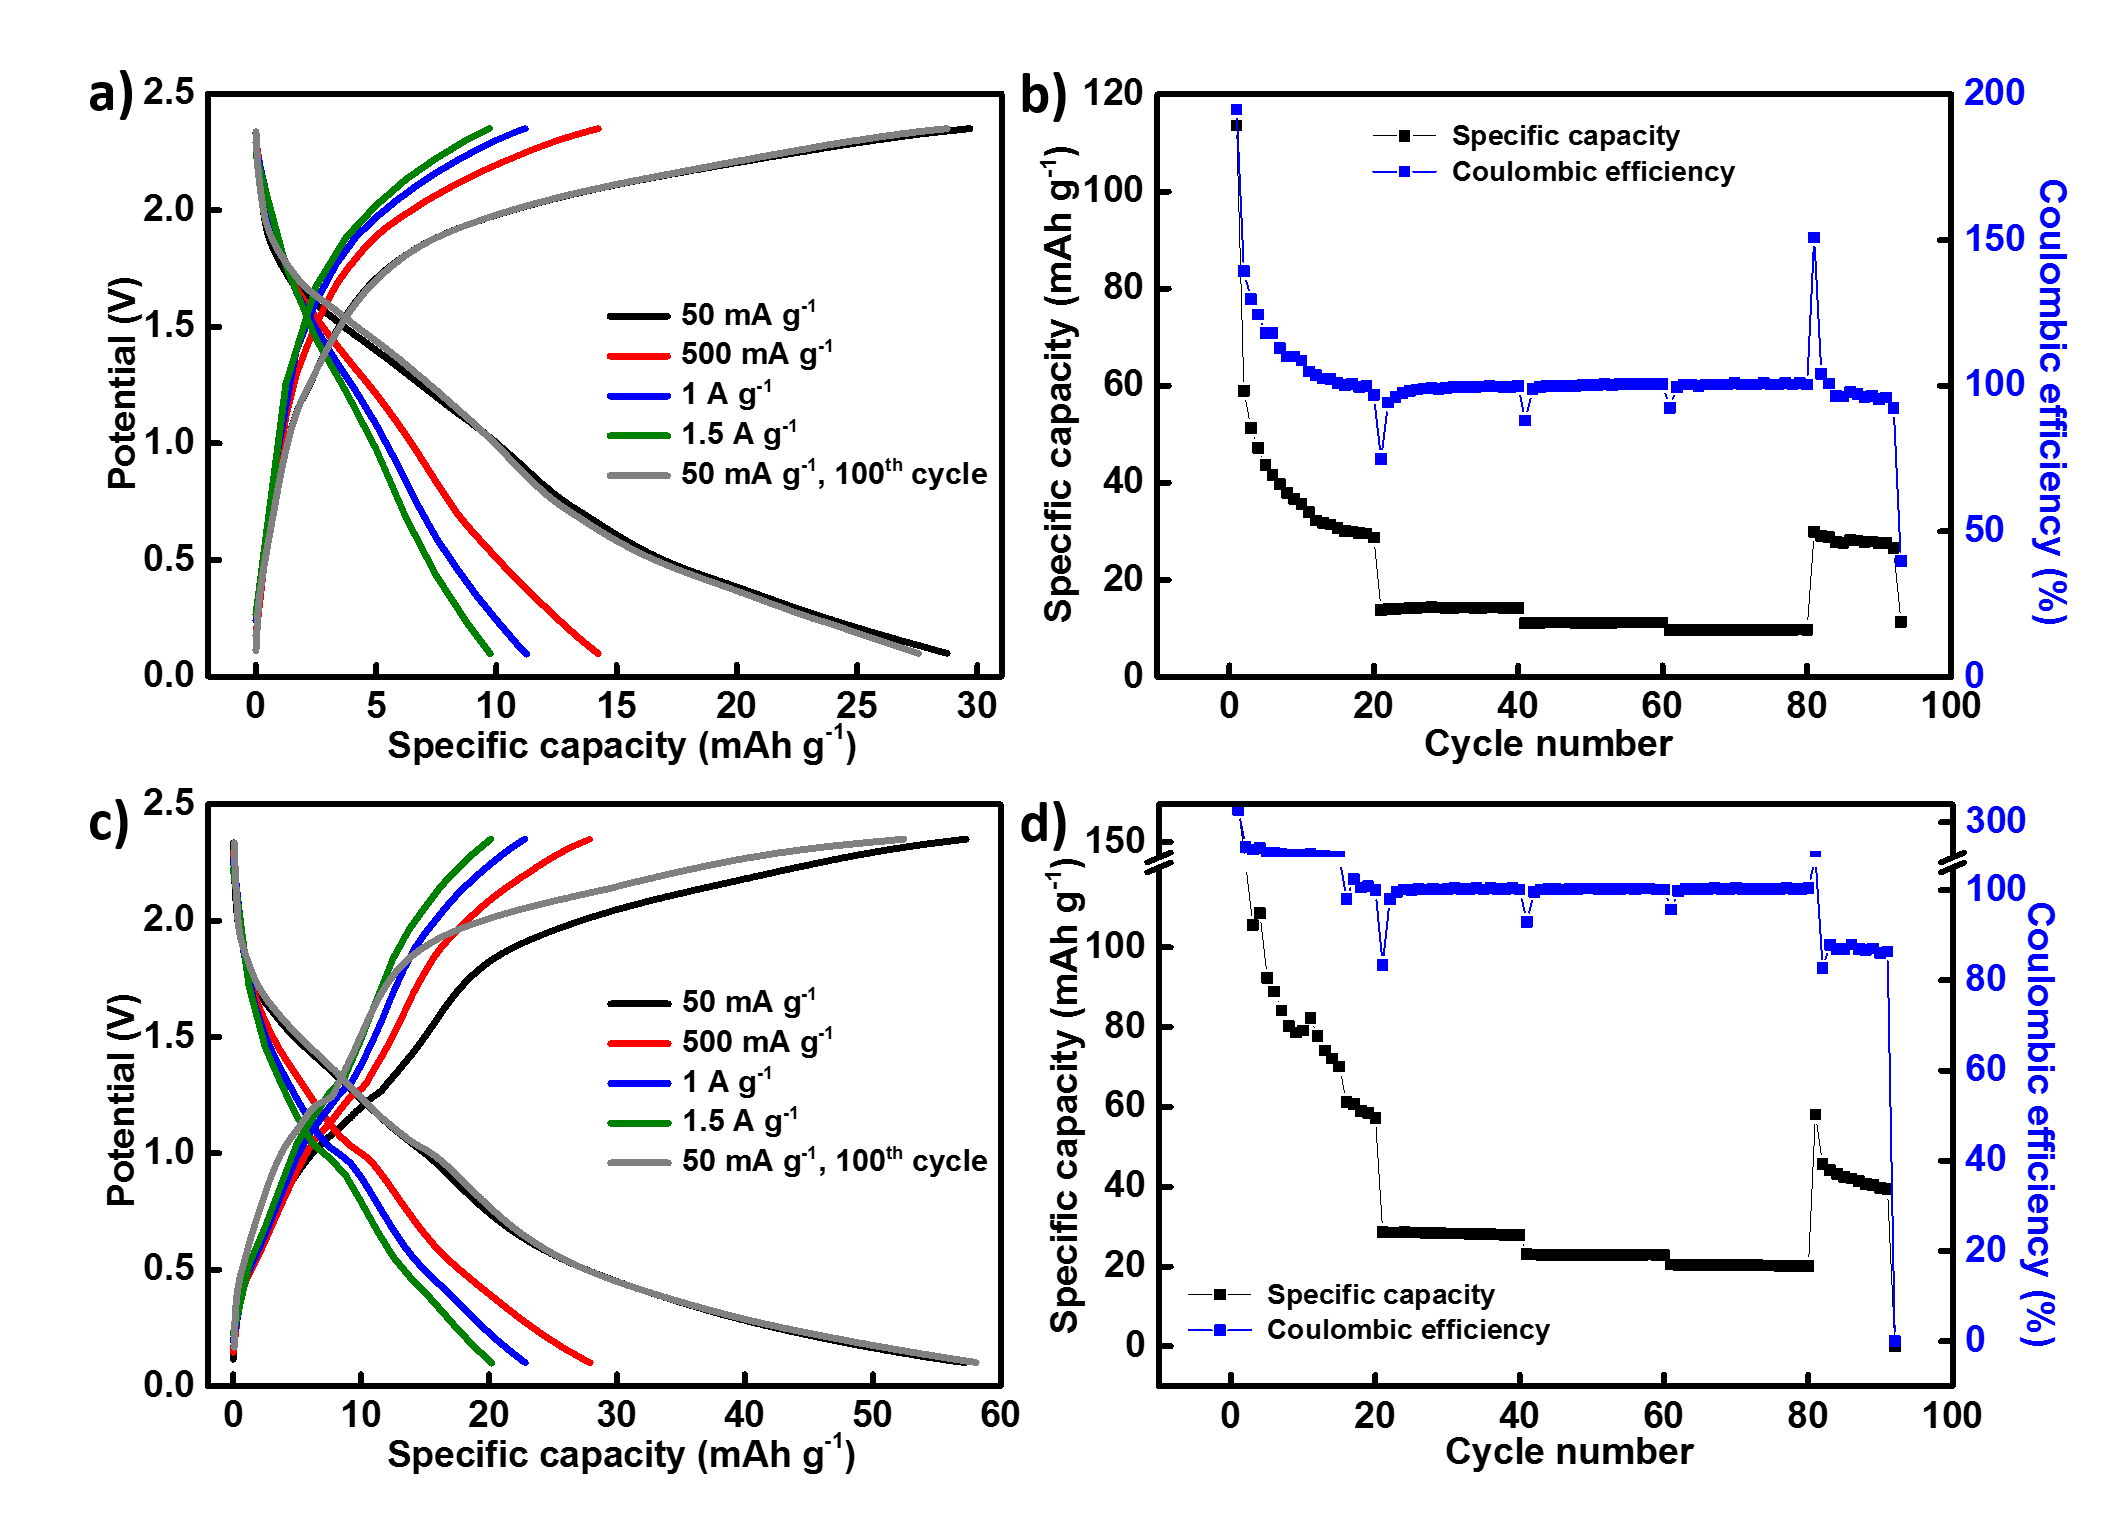
\includegraphics[width=\textwidth]{Figures/BOhBN/BNdifO}
\caption{Galvanostatic charge/discharge profile and cell efficiencies of AIBs composed of a-b) \ce{hBN}/\ce{MnO2} and c-d) \ce{TiO2}/hBN cathodes.}
\label{Figures/BOhBN:BNdifO}
\end{figure}

A few other combinations were tested as cathodes and the results are displayed in Figure \ref{Figures/BOhBN:othON}.

\begin{figure}[tbh!]
\centering
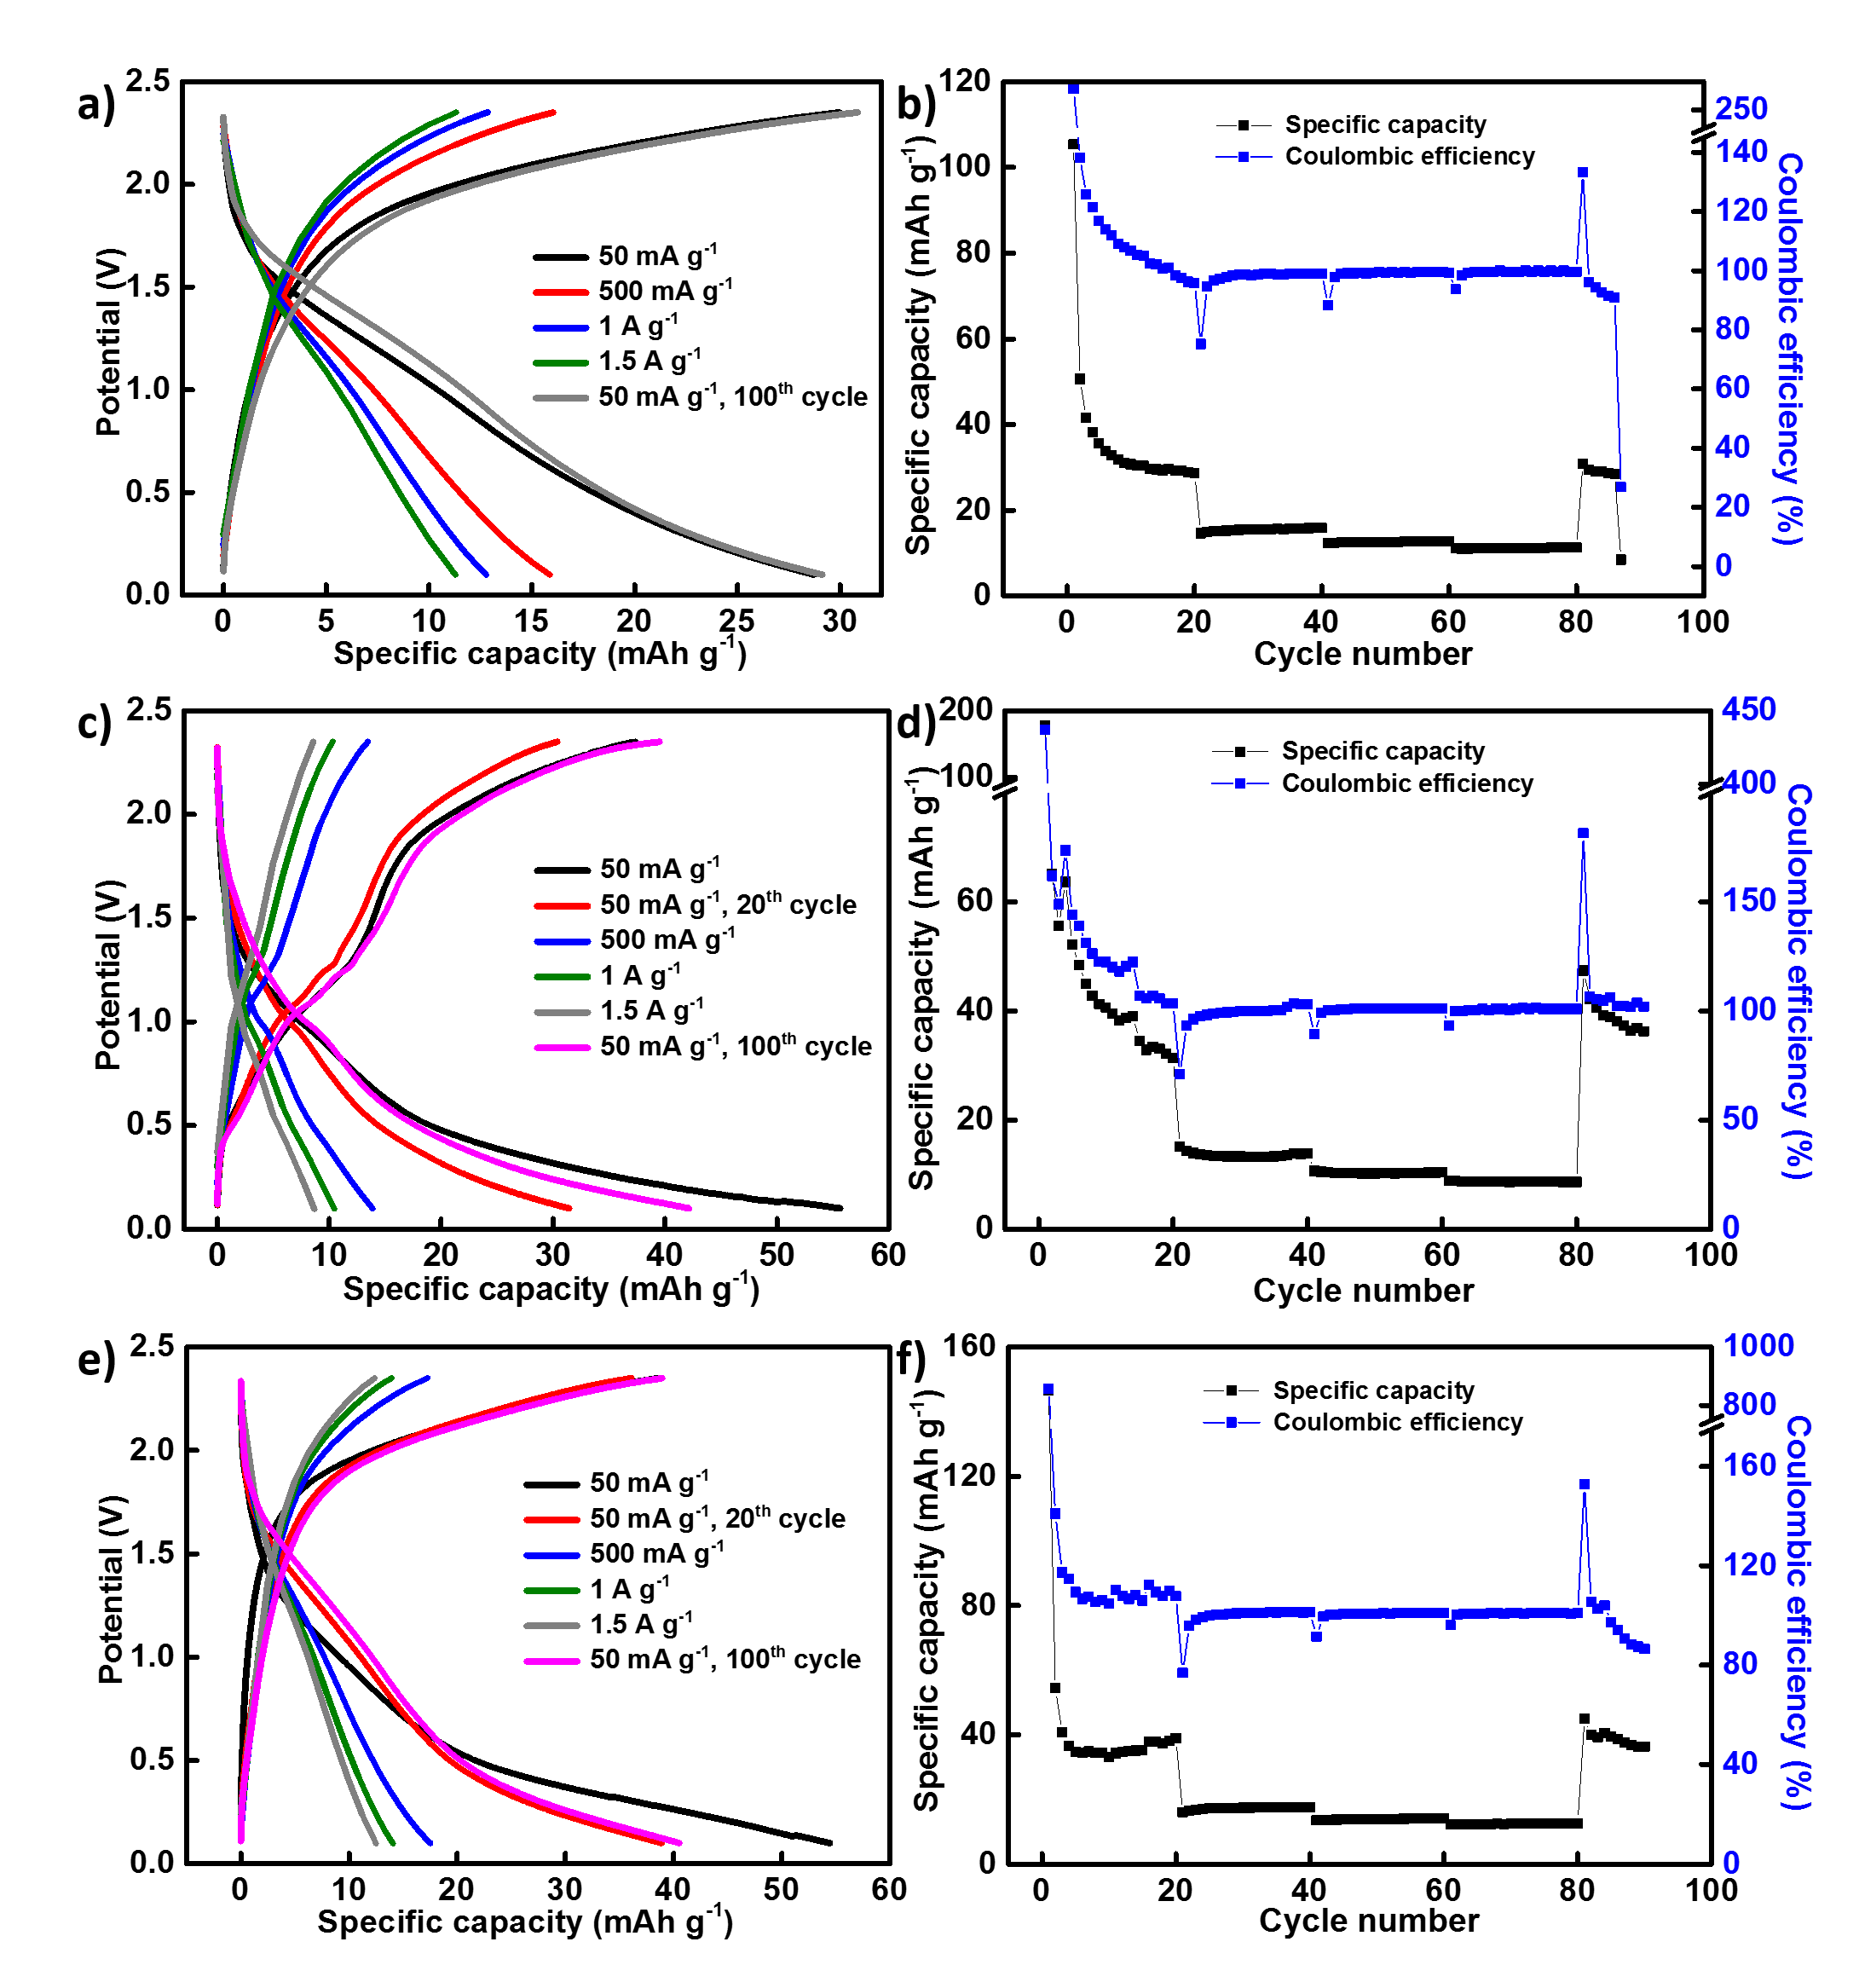
\includegraphics[width=\textwidth]{Figures/BOhBN/othON}
\caption{Galvanostatic charge/discharge profile and cell efficiencies of AIBs composed of a-b) \ce{MnO2}/\ce{C3N4} c-d) \ce{TiO2}/\ce{C3N4} and e-f) \ce{MnO2}/\ce{Si3N4} cells.}
\label{Figures/BOhBN:othON}
\end{figure}

The research findings from this chapter raises a lot of questions that need to be answered.
\begin{itemize}
    \item {\Large{Role of hBN.}} Is it only providing structural support to \ce{B2O3} or is it actually participating actively in the electron transfer process? If this is just a conversion reaction and hBN is not playing any significant role, why do other nitrides when combined with \ce{B2O3}, do not produce high discharge capacity $\sim$ 250 mAh g$^{-1}$?
    \item {\large{First principle studies of hBN/\ce{B2O3}.}} A conversion-type reaction has been hypothesised for this new material. However, it is important to study the changes taking places inside the cell \textit{in-situ} to fully determine the cell's mechanism. 
    \item {\Large{Using other nitrides and oxides.}} Once the role of nitrides and oxides in this mixture is established, can cheaper alternatives be used instead of hBN? On that note, why do the results in Table \ref{tabdiffpc} differ so much?
\end{itemize}

